\chapter{Numerical Simulations}
\lettrine{T}{he} present chapter describes the performances and limitations of the proposed visual navigation pipeline based on the results of numerical simulations.\\
Using the testing framework described in \cref{sec:testing}, the algorithm was stressed in various conditions to understand its advantages and limitations. The testing plan followed is reported in \cref{tab:testplan}, where the different cases for the illumination conditions are presented in \cref{tab:ill_cases}. \\

\begin{table}[!h]

    \centering
    \begin{tabular}{p{1.5cm} p{2.5cm} p{2.5cm} p{7.3cm}}
        Test n. & Illumination condition &  Spectra  & Scope  \\
        \hline \hline
        1 & Case A & VIS \& TIR  & \multirow{3}{*}{\parbox{7.3cm}{Evaluate the nominal performances of the multispectral filter, comparing them to the VIS-only and TIR-only applications. (Research questions 1,2)}} \\ 
        &  & VIS & \\ 
        &   & TIR & \\ \hline
        2 & Cases B,C & VIS \& TIR & Evaluate the robustness to low illumination for multispectral navigation. (Research questions 1,2)\\ \hline
        3 & Cases B,D & TIR &  Evaluate the robustness of TIR-only navigation under both sunlit and eclipse conditions. (Research question 3)\\ \hline
        4 & Case A & VIS \& TIR & Varying relative distance ($\SI{20}{m}$ to $\SI{80}{m}$) to assess the range of applicability of the visual navigation pipeline in terms of chaser-target distance.\\ \hline
        5& Case A & VIS \& TIR & Synchronous chaser-target rotation to evaluate the influence of apparent dynamics in the visual navigation pipeline. \\ \hline
    \end{tabular}
    \caption{Test plan and rationale}
    \label{tab:testplan}
\end{table}
\newpage
At first, the filter's effectiveness is tested in a nominal condition, evaluating the advantages of sensor fusion when both the thermal and visible spectra provide good data quality.
Secondly, different aspects of the pipeline are stressed, starting with its dependability from illumination conditions. The possibility of TIR-only navigation is investigated to overcome the aforementioned criticality, presenting its applicability to the test case.
Finally, the navigation pipeline robustness is tested against the chaser-target distance and a condition of synchronous rotation. \\
A comparative assessment is qualitatively performed concerning image fusion techniques applied to navigation about small bodies, as it represents a valuable alternative to the proposed method.

\section{Test 1: nominal performances }
\chaptermark{Numerical Simulations}
At first, the visual navigation pipeline performances are evaluated in favorable illumination conditions (Case A), having a good target illumination with a phase angle of $\SI{25}{\deg}$ and a distance of $\SI{35}{\meter}$, which do not compromise the Image Processing pipeline as the target is well illuminated and clearly visible on the image plane.\\
The conditions in which Test 1 is performed are reported in \cref{tab:contest1}.\\

\begin{table}[!h]
    \centering
    \begin{tabular}{C{1.8cm} C{1.8cm} C{4cm}}
     $\phi$ & $\rho$ & Relative distance\\ \hline\hline
     $\SI{25}{\deg}$ & $>\SI{0}{\deg}$ & $\SI{35}{\meter}$\\\hline
   
    \end{tabular}
    \caption{Test 1 illumination conditions and relative distance}
    \label{tab:contest1}
\end{table}

The trajectory followed by the chaser about the target expressed in the target body and LVLH frame is reported in \cref{fig:track}.

\begin{figure}[!h]
    \begin{subfigure}[b]{0.48\textwidth}
    \centering
    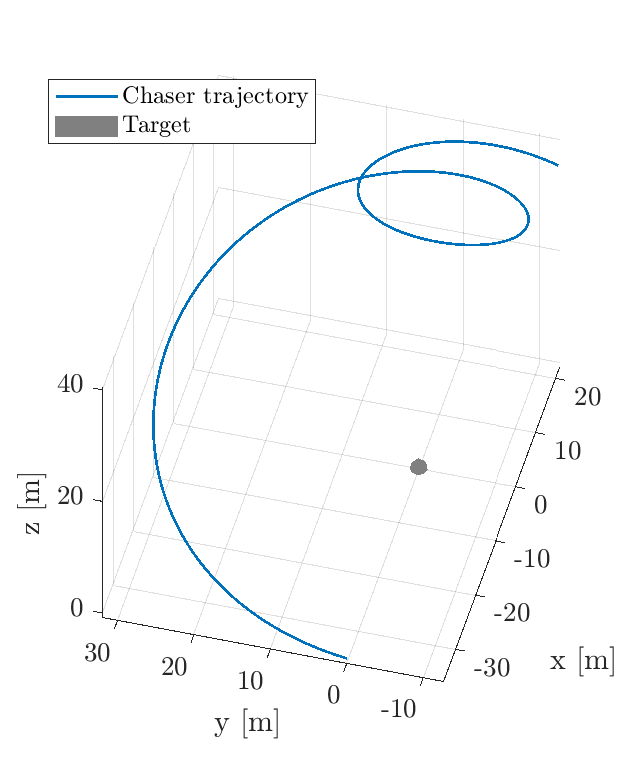
\includegraphics[clip,trim = 0cm 0cm 0cm 1cm,width=\linewidth]{Images/bodyttraj.eps}
    \caption{Target body frame}
    \label{fig:trajbody}
    \end{subfigure}\hfill
    \begin{subfigure}[b]{0.48\textwidth}
    \centering
    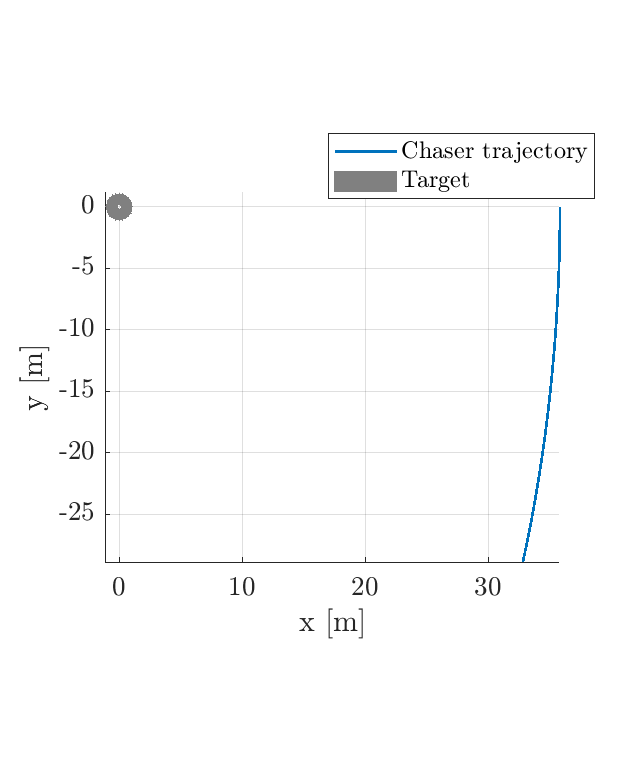
\includegraphics[clip,trim = 0cm 2cm 0cm 1cm,width=\linewidth]{Images/lvlhttaj.eps}
    \caption{Target LVLH frame}
    \label{fig:trajLVLH}
    \end{subfigure}
    \caption{Chaser trajectory in target's body frame and LVLH frame}
    \label{fig:trak}
\end{figure}
As the thesis work does not include the pose acquisition routine, the initialization of the filter is performed assuming an initial error with respect to the ground truth in terms of position and attitude. The amplitude of the error is selected to be consistent with the results of \cite{pesce2019autonomous}, randomly generating a position offset in the order of \SI{1}{\meter}, and an attitude variation of $\SI{8}{\deg}$ maximum. Since the pose acquisition process does not provide information regarding the initial values of the relative velocity or the angular rates, these states are initialized to zero in the filter. The states initialization prior to the addition of the randomic initialization errors is reported in \cref{tab:posinit1,tab:attinit1} for the position and attitude parameters. In \cref{tab:attinit1} the attitude is parameterized in Euler angles (X $\psi$, Y $\phi$, Z $\theta$) to provide a more straightforward physical interpretation with respect to quaternions.\\

\begin{table}[!h]
    \centering
    \begin{tabular}{ c c c c c c}
        $x$ & $y$ & $z$ & $\dot{x}$ & $\dot{y}$ & $\dot{z}$ \\\hline\hline
        $\SI{35}{\meter}$ & $\SI{0}{\meter}$ & $\SI{0}{\meter}$ & $\SI{0}{\meter\per\second}$ & $\SI{0}{\meter\per\second}$ & $\SI{0}{\meter\per\second}$  \\\hline
    \end{tabular}
    \caption{Relative velocity and position initialization}
    \label{tab:posinit1}
\end{table}
\begin{table}[!h]
    \centering
    \begin{tabular}{c c c c c c}
         $\psi$ & $\phi$ & $\theta$ & $\omega_x$ & $\omega_y$ & $\omega_z$\\\hline\hline
         $\SI{0}{\deg}$ & $\SI{0}{\deg}$ & $\SI{0}{\deg}$ & $\SI{0}{\deg\per\second}$  & $\SI{0}{\deg\per\second}$   & $\SI{0}{\deg\per\second}$ \\\hline
    \end{tabular}
    \caption{Relative attitude and angular rates initialization}
    \label{tab:attinit1}
\end{table}

Both the states' covariance matrix and the process noise covariance matrix are initialized as diagonal matrices. The diagonal elements of the matrix are defined for each state and reported in \cref{tab:PQinit}.
As for the covariance matrix, the values are defined to be noticeably higher than the covariance estimate computed by the filter reached steady state. This is performed to account for the initialization error and perform a faster filter convergence to the correct values in the first steps. Considering the filter's dynamic truthfulness, the process noise covariance matrix has been defined with a trial and error procedure to enhance the filter's performance. For the tuning of $\vect{Q}$, its influence on the covariance estimation is also considered, trying to avoid either under or over-estimating the states' uncertainty.\\
\begin{table}[!h]
    \begin{subtable}[h]{0.45\textwidth}
        \centering
        \begin{tabular}{l  c c}
        Parameter & Value & Unit\\ \hline \hline
        $\sigma_{\vect{x}}^2 $ & $\expnumber{2.5}{+0}$ & \SI{}{\meter^2}\\\hline
        $\sigma_{\dot{\vect{x}}}^2 $ & $\expnumber{8.0}{-2}$ & \SI{}{\meter^2\per\second^2}\\\hline
        $\sigma_{\vect{a}_p}^2 $ & $\expnumber{1.0}{-2}$ & /\\\hline
        $\sigma_{\omega}^2 $ & $\expnumber{2.0}{-2}$ & \SI{}{\radian^2\per\second^2}\\\hline
        \end{tabular}
        \caption{Initial covariance matrix settings}
        \label{tab:P0}
     \end{subtable}\hfill
    \begin{subtable}[h]{0.45\textwidth}
        \centering
        \begin{tabular}{l  c c}
        Parameter & Value & Unit\\ \hline \hline
        $\sigma_{\vect{x}}^2 $ & $\expnumber{2.5}{+0}$ & \SI{}{\meter^2}\\\hline
        $\sigma_{\dot{\vect{x}}}^2 $ & $\expnumber{5.0}{-6}$ & \SI{}{\meter^2\per\second^2}\\\hline
        $\sigma_{\vect{a}_p}^2 $ & $\expnumber{3.0}{-3}$ & /\\\hline
        $\sigma_{\omega}^2 $ & $\expnumber{6.0}{-4}$ & \SI{}{\radian^2\per\second^2}\\\hline
        
       \end{tabular}
       \caption{Process noise covariance diagonal elements}
       \label{tab:Q0}
    \end{subtable}
     \caption{Diagonal values of the matrices $\vect{Q}$ and $\vect{P}$ at the initial step of the filter}
     \label{tab:PQinit}
\end{table}
Although the measurement noise matrix $\vect{R}$ is estimated online by the filter, it is required to provide an initialization as it is estimated recursively. The initial values were set to be close to the estimates performed by the $\vect{R}$-adaptation routine to ensure good performances and avoid numerical issues. Similarly to $\vect{P}$ and $\vect{Q}$, the measurement noise covariance matrix is initialized as a diagonal matrix, whose diagonal elements are reported in \cref{tab:R0}. The values are expressed in pixels and refer to non-rectified images, as the measurements are modeled with a pinhole camera model. This is not considered a critical point as  the rectification is taken into account by the calibration of the camera in real applications. 
\begin{table}[!h]
    \centering
        \begin{tabular}{l  c c}
        Parameter & Value & Unit\\ \hline \hline
        $\sigma_{VIS} $ & $20$ & \SI{}{\pixel}\\\hline
        $\sigma_{TIR} $ & $10$ & \SI{}{\pixel}\\\hline
        \end{tabular}
        \caption{Initial standard deviation assigned to the features}
    \label{tab:R0}
\end{table}
Given these initialization parameters, the algorithm has been tested on a database of four hundred synthetic images generated along the trajectory reported in \cref{fig:track}. The filter's operating frequency has been set to be $\SI{1}{\hertz}$. The navigation pipeline has been tested by feeding both the VIS and TIR, the visible only, and the thermal only information in the navigation filter.
%on the fused VIS and TIR information, the visible images only, and using the thermal images only. 
The results of position and attitude errors for a single run, defined as presented in \cref{sec:errors}, are reported in \cref{fig:err_pos,fig:err_att} respectively.\\
\begin{figure}[!h]
    \begin{subfigure}[b]{1\textwidth}
    \centering
    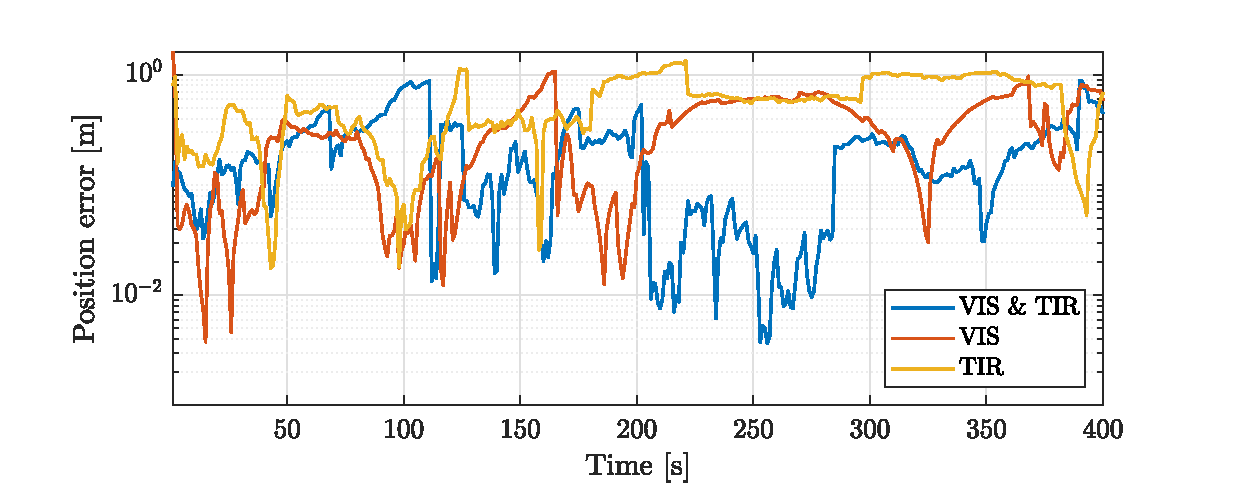
\includegraphics[width=0.93\linewidth]{Images/pos_err_corrected.eps}
    \caption{Position AKE}
    \label{fig:err_pos}
    \end{subfigure}\hfill
    \begin{subfigure}[b]{1\textwidth}
    \centering
    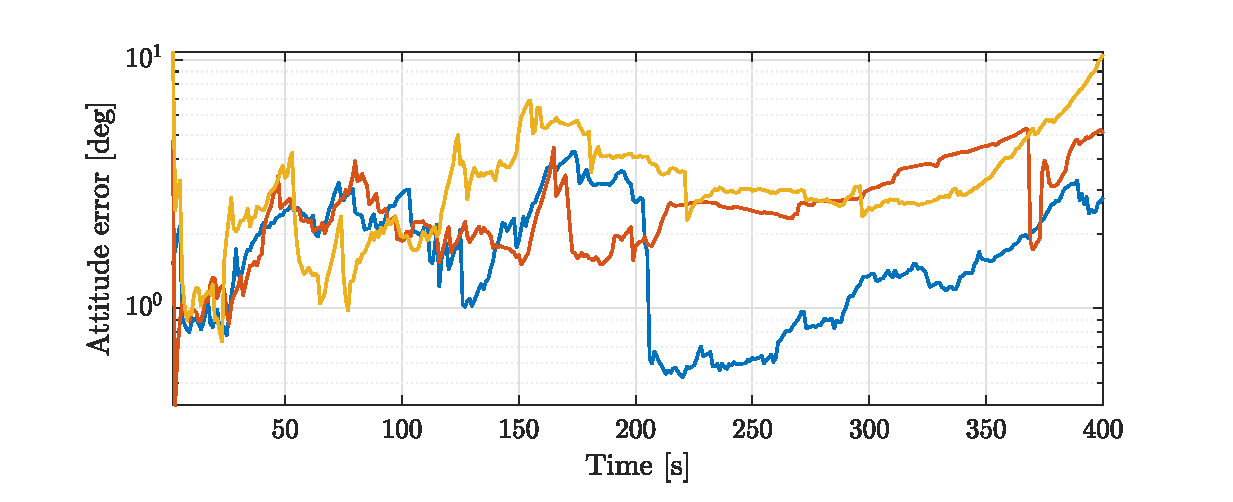
\includegraphics[width=0.93\linewidth]{Images/att_err_corrected.eps}
    \caption{Attitude AKE}
    \label{fig:err_att}
    \end{subfigure}
    \caption{Position and attitude errors over a 400 seconds simulation}
    \label{fig:err_posatt}
\end{figure}
From \cref{fig:err_pos,fig:err_att}, it can be qualitatively assessed that the multispectral case can track the position and attitude without ever diverging through the simulation. The multispectral information proved to provide consistently better results than the VIS-only or TIR-only case, as understandable also from the numerical values reported in \cref{tab:posatters}. This result was expected as in the multispectral case the filter has more information coming from the sensors, thus it can provide a better estimate of the states. \newline
\begin{table}[!h]
    \begin{subtable}[h]{1\textwidth}
        \centering
        \begin{tabular}{l  c c}
        Spectrum & Absolute MKE [$\SI{}{\meter}$]& Relative MKE [\%]\\ \hline \hline
        VIS \& TIR &$0.25\pm 0.18$ & $0.63\pm 0.54$\\\hline
        VIS & $0.35\pm 0.21$ & $0.85\pm 0.60$\\\hline
        TIR & $0.59\pm 0.29$ & $1.51\pm 0.82$\\\hline
        
       \end{tabular}
       \caption{Position errors}
       \label{tab:poserrs}
    \end{subtable}
    \hfill
    \begin{subtable}[h]{1\textwidth}
        \centering
        \begin{tabular}{l  c }
        Spectrum & Absolute MKE [$\SI{}{\deg}$]\\ \hline \hline
        VIS \& TIR &  $1.72\pm 0.88$\\\hline
        VIS &  $2.64\pm 1.04$ \\\hline
        TIR &  $3.36\pm 1.66$ \\\hline
        \end{tabular}
        \caption{Attitude errors}
        \label{tab:atterrs}
     \end{subtable}
     \caption{Position and attitude errors for the different spectrum modalities}
     \label{tab:posatters}
\end{table}
The chaser's estimated trajectory of the chaser in the target body frame, affected by both the position and attitude errors, is represented in \cref{fig:estrajectory}. It can be observed how, after the initial correction of the initialization offset, the estimated path remains bounded to the ground truth on which the sensor's output has been generated. \\

\begin{figure}[!h]
    \centering
    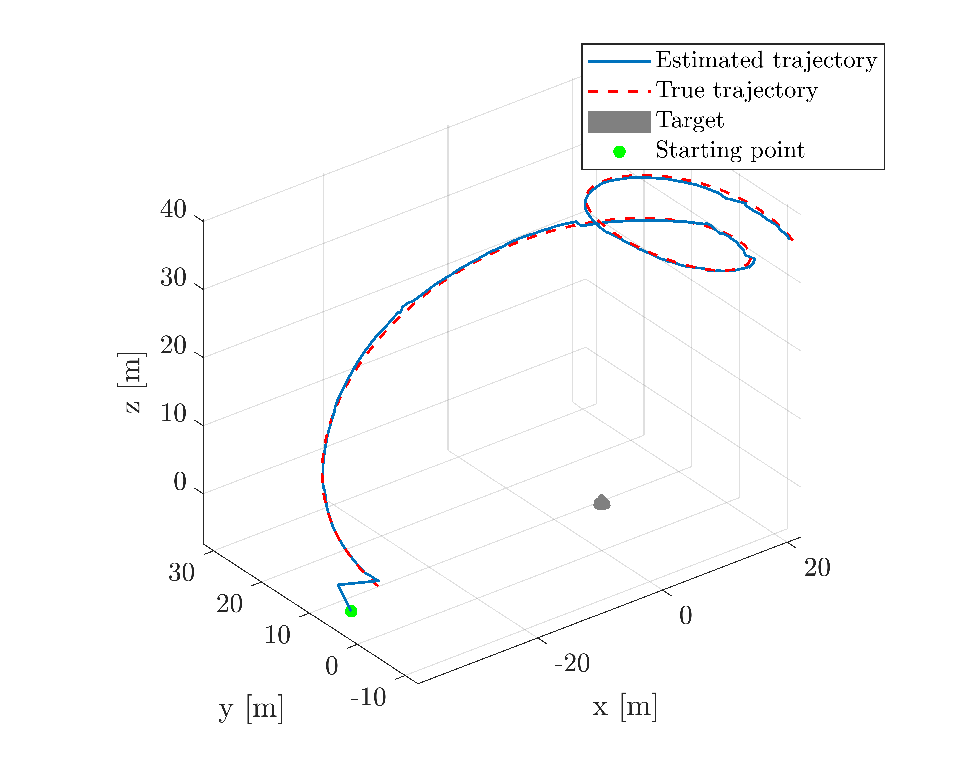
\includegraphics[width = 0.8\linewidth]{Images/esttraj.eps}
    \caption[Ground truth and estimated trajectory]{Ground truth and estimated trajectory of the chaser about the target body frame}
    \label{fig:estrajectory}
\end{figure}
To discuss the confidence in the states' estimation, the position and attitude errors are reported for each component with the associated uncertainty expressed in $3\sigma$. \cref{fig:sigma_posatt} shows that the filter provides a reliable estimation of both the relative position and attitude, as the confidence region envelopes the errors without overestimating the uncertainty. The sudden drops in the standard deviation correspond to the re-initialization steps. That is an expected behavior as the uncertainty increase with the decrease in number of features and reduces whenever new features are added.\newline
\begin{figure}[!h]
    \begin{subfigure}[b]{0.48\textwidth}
    \centering
    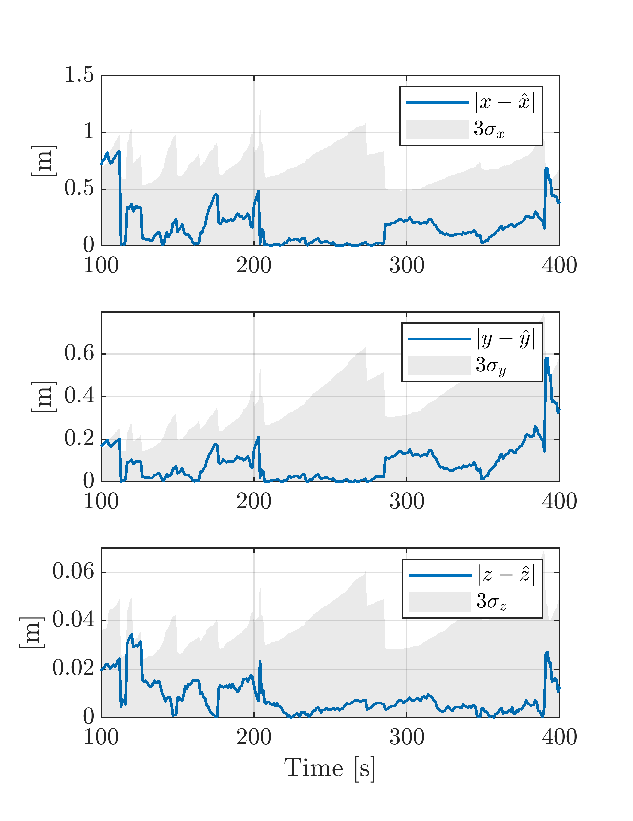
\includegraphics[width=\linewidth]{Images/sigmapos.eps}
    \caption{Position}
    \label{fig:sigma:pos}
    \end{subfigure}\hfill
    \begin{subfigure}[b]{0.48\textwidth}
    \centering
    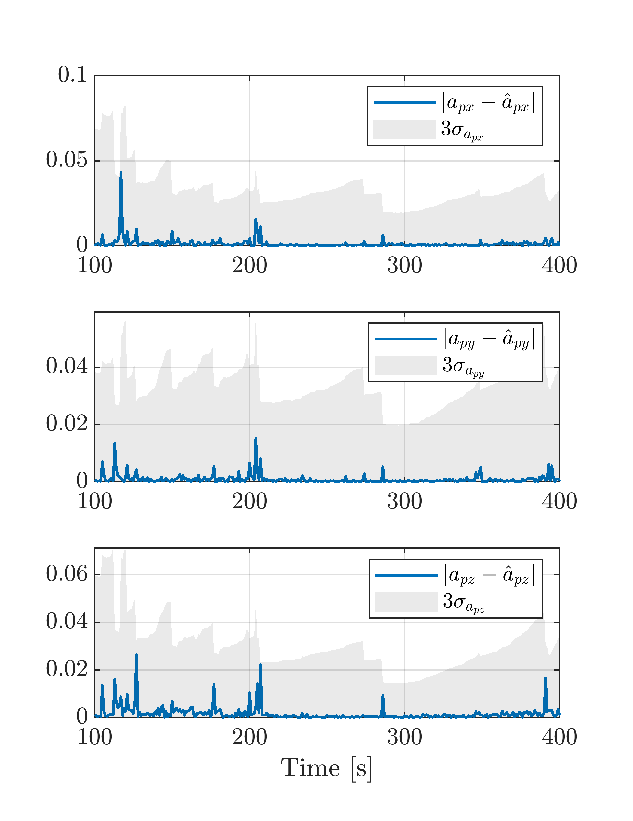
\includegraphics[width=\linewidth]{Images/sigmaatt.eps}
    \caption{Attitude (MRP)}
    \label{fig:sigma_att}
    \end{subfigure}
    \caption{Difference between the true and estimated position and attitude (MRP) states with associated uncertainty}
    \label{fig:sigma_posatt}
\end{figure}
As the attitude error state expressed in Modified Rodriguez Parameters (\cref{fig:sigma_att}) does not provide a straightforward physical representation of the problem, the true and estimated Euler angles associated with the relative attitude are reported in \cref{fig:eulerangles} for completeness. The rotation sequence is X ($\psi$), Y ($\phi$), Z ($\theta$).\newline
\begin{figure}[!h]
    \centering
    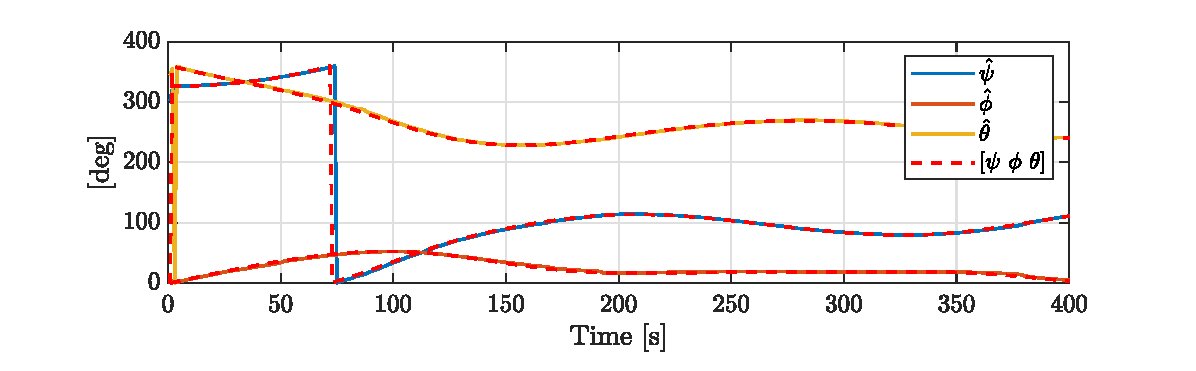
\includegraphics[width = \linewidth]{Images/eulerangles.eps}
    \caption[True and estimated Euler angles]{True and estimated Euler angles according to XYZ rotation sequence ($\ \hat{\cdot} \ $ indicates the estimated values)}
    \label{fig:eulerangles}
\end{figure}
The same representation of \cref{fig:sigma_posatt} is reported for the relative velocities and angular rates in \cref{fig:sigmavel,fig:sigmarate}, respectively. The visualization starts at $\SI{100}{\second}$ to enhance the understanding of the graphical representation that would be otherwise compromised by the high error values given by the initialization errors. For both the relative velocities and angular rates, an overestimation of the covariance and an almost null dependence on the feature re-initialization appear evident, contrarily to the relative position or attitude case. This latter phenomenon is justified by the fact that there is no direct measurement of the velocity and angular rates. \\
The uncertainty region associated with the relative velocities decreases as it converges after the initial overestimation due to the initialization error, although presenting a very slow convergence to the steady state value. On the other hand, the overestimation of the relative angular rates results from the increased value of its process noise covariance matrix. Because of the filter's dynamic unreliability, a higher entrustment of the propagated value would result in a higher error.  \newline
\begin{figure}[!h]
    \begin{subfigure}[b]{0.48\textwidth}
    \centering
    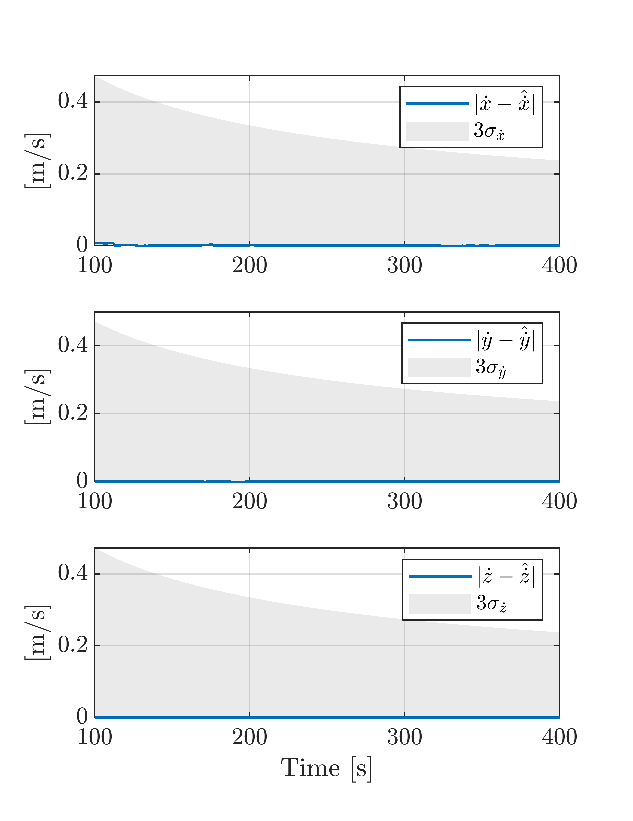
\includegraphics[clip,trim = 0cm 0cm 0cm 0cm,width=\linewidth]{Images/sigma_vel.eps}
    \caption{Velocity}
    \label{fig:sigmavel}
    \end{subfigure}\hfill
    \begin{subfigure}[b]{0.48\textwidth}
    \centering
    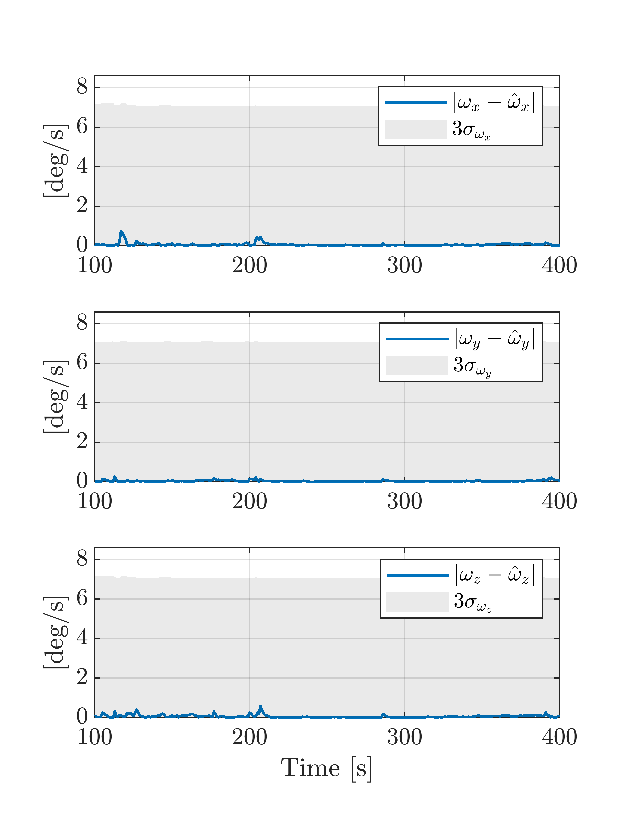
\includegraphics[clip,trim = 0cm 0cm 0cm 0cm,width=\linewidth]{Images/sigma_rate.eps}
    \caption{Angular rates}
    \label{fig:sigmarate}
    \end{subfigure}
    \caption{Difference between the true and estimated relative velocities and angular rates with associated confidence region}
    \label{fig:sigmavelrate}
\end{figure}
The measurement noise matrix adaptation results are reported in \cref{fig:colors}, graphically illustrating the variance values of the model features at the end of the simulation for both the visible and thermal spectrum. \cref{fig:colors} shows how the visible and thermal spectra differ in variance values and which features have been matched by the IP routine. As detailed in the following analysis, those differences are one of the reasons behind the TIR spectrum lower performance. \\

\begin{figure}[!h]
    \centering
    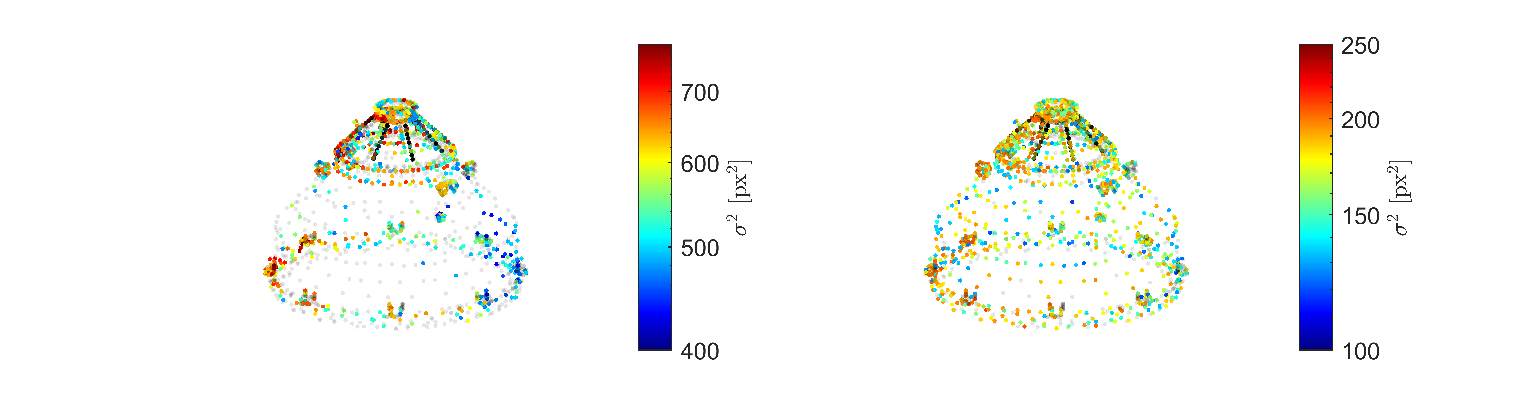
\includegraphics[clip,trim = 2cm 0cm 1cm 0cm,width=\linewidth]{Images/colors2.eps}
    \caption[Variance of the features at the end of the simulation]{Variance of the features at the end of the simulation for VIS (left) and TIR (right) images}
    \label{fig:colors}
\end{figure}
As the filter works at a frequency of $\SI{1}{\hertz}$, the algorithm must have a computational time smaller than the filter's update time. The computation time of the filter steps and the re-initialization process are reported in \cref{tab:Csteps,tab:Creinit} respectively. Those results are obtained on a Desktop PC with processor Intel Core i5-7300HQ 4 x 2.5 GHz.\\
The filter run time remains well under one second in all three cases. Since the operations must be performed twice, the multispectral application is almost twice as slow as single-spectrum cases. The re-initialization time is critical, as the computational time is prohibitive as it greatly exceeds the filter's operating frequency of $\SI{1}{\hertz}$. \\
The presented times must be reevaluated on relevant hardware to understand the onboard applicability; however, at the current stage, the computational burden is identified as a critical point of the proposed pipeline.
\begin{table}[!h]
    \begin{subtable}[h]{0.42\textwidth}
        \centering
        \begin{tabular}{l  c }
        Spectrum & CPU Time [$\SI{}{\second}$]\\ \hline \hline
        VIS \& TIR &  $0.17\pm 0.03$\\\hline
        VIS &  $0.08\pm 0.02$ \\\hline
        TIR &  $0.07\pm 0.02$ \\\hline
        \end{tabular}
        \caption{Filter's step computational time}
        \label{tab:Csteps}
     \end{subtable}
    \hfill
    \begin{subtable}[h]{0.42\textwidth}
        \centering
        \begin{tabular}{l  c }
        Spectrum & CPU Time [$\SI{}{\second}$]\\ \hline \hline
        VIS &  $8.9\pm 0.55$ \\\hline
        TIR &  $9.0\pm 0.46$ \\\hline
        \end{tabular}
        \caption{re-initialization computational time}
        \label{tab:Creinit}
     \end{subtable}
     \caption{CPU time for the the filter step and the reinitialization process}
     \label{tab:Ctimes}
\end{table}
\section{Navigation pipeline limitations}
\chaptermark{Numerical Simulations}
In the following sections, the visual navigation filter is tested in different conditions (Test 2-5 of \cref{tab:testplan}) to assess its limitations and range of applicability. The different testing conditions are presented, and the obtained results are discussed to identify the shortcoming and propose possible mitigations.

\subsection{Test 2: low illumination conditions}
A well-known VIS cameras limitation is the dependence on the target illumination conditions. To assess this condition the algorithm was tested on a database of one-hundred images generated with a phase angle close to $\SI{100}{\deg}$. In this condition, most of the target is shadowed, and the low quality information coming from the VIS sensors limits the filter performances. A frame of the rendered database is reported in \cref{fig:frame215}, as an example.\\
The environmental conditions in which the simulation is performed are summarized in \cref{tab:contest2}.\\

\begin{table}[!h]
    \centering
    \begin{tabular}{C{1.8cm} C{1.8cm} C{4cm}}
     $\phi$ & $\rho$ & Relative distance\\ \hline\hline
     $\SI{100}{\deg}$ & $>\SI{0}{\deg}$ & $\SI{35}{\meter}$\\\hline
   
    \end{tabular}
    \caption{Test 2 illumination conditions and relative distance}
    \label{tab:contest2}
\end{table}

The obtained results in terms of position and attitude errors are reported in \cref{fig:lowillerrors}: the low illumination conditions strongly affect the results, causing a strictly increasing error in terms of attitude and deteriorating the performance in terms of position estimation. The exceedingly high errors emphasize that the multispectral data-fusion is not suitable for low illumination conditions.\\

\begin{figure}[!h]
    \begin{subfigure}{0.48\linewidth}
    \centering
    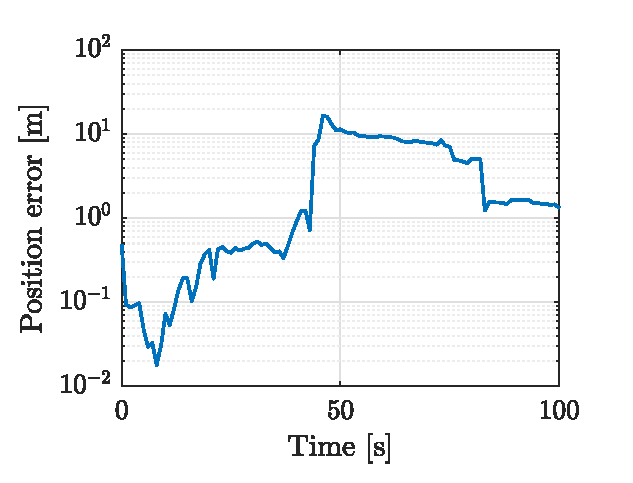
\includegraphics[width = 1\linewidth]{Images/lowillpos.eps}
    \caption{Position AKE}
    \label{fig:lowillpos}
    \end{subfigure}\hfill
    \begin{subfigure}{0.48\linewidth}
    \centering
    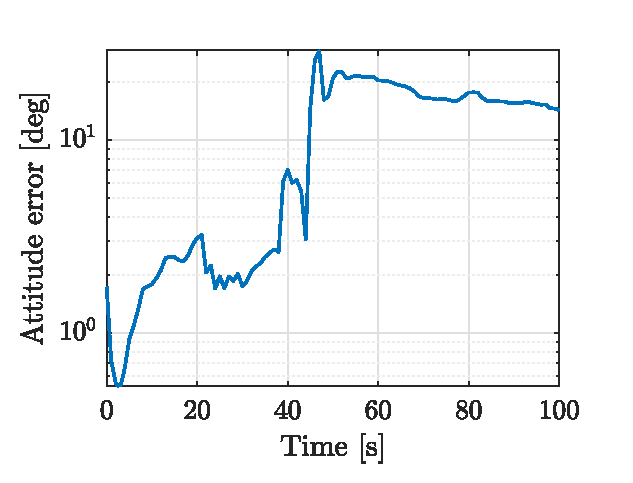
\includegraphics[width = 1\linewidth]{Images/lowillatt_corrected.eps}
    \caption{Attitude AKE}
    \label{fig:lowillatt}
    \end{subfigure}
    \caption{Position and attitude errors in case of low illumination conditions}
    \label{fig:lowillerrors}
\end{figure}

The low-quality data provided by the visible sensor have a counterproductive effect on the estimation process, increasing the number of outliers in the measurements and forcing a continuous re-initialization of the features. A small region of the target illuminated decreases the number of features detected in the visible images and concentrates them on a small region of the target, making the pose correction step less effective and affecting it negatively.\\
As already discussed in \cref{sec:rendering}, a scarce illumination affecting the visible camera is caused both from an high phase angle (\cref{fig:frame215}) and by a low elevation angle $\rho$  (\cref{fig:frame022}), as the concavity is almost always shadowed.\\
% Investigating the sources of errors in the Image Processing routine, a double correlation was identified between the number of features detected by the ORB detector and both the illumination condition of the target (\cref{fig:frame215}) and the elevation of the chaser with respect to the target body frame (\cref{fig:frame022}).

\begin{figure}[!h]
    \begin{subfigure}{0.48\linewidth}
    \centering
    \includegraphics[width = 0.75\linewidth]{Images/frame_00215.png}
    \caption{Sample image in low illumination conditions}
    \label{fig:frame215}
    \end{subfigure}\hfill
    \begin{subfigure}{0.48\linewidth}
    \centering
    \includegraphics[width = 0.75\linewidth]{Images/frame_00022.png}
    \caption{Detail of VESPA concavity}
    \label{fig:frame022}
    \end{subfigure}
    \caption{Examples of unfavourable visible conditions}
    \label{fig:lowillimages}
\end{figure}
This aspect was further investigated highlighting how it affects the feature detection process. \cref{fig:illelcorr} highlights how the illumination angle is as influential as the chaser elevation angle. It is observed that the only reliable condition is represented by a low phase angle and a high elevation angle. \\

\begin{figure}[!h]
    \centering
    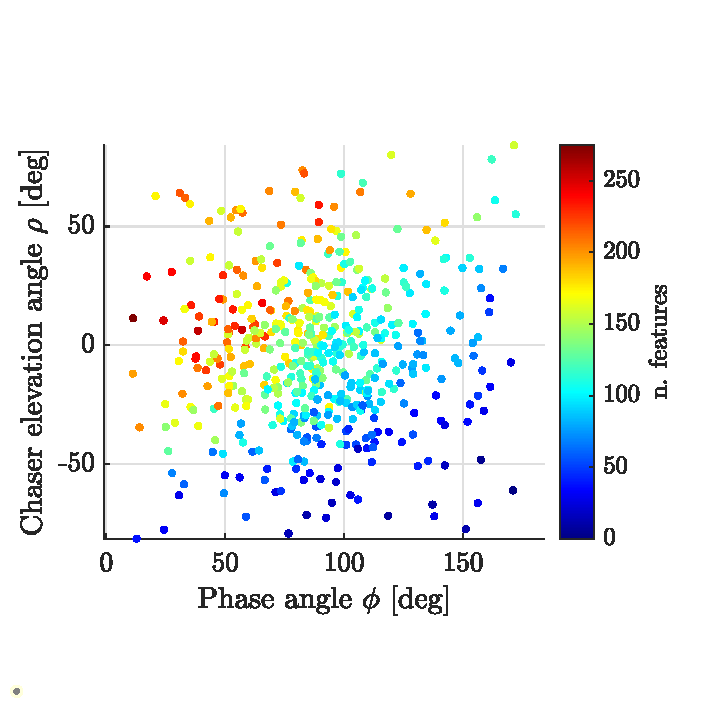
\includegraphics[clip, trim = 0cm 1cm 0cm 1cm, width = 0.5\linewidth]{Images/suninclcorr.eps}
    \caption[Feature detection dependability on $\rho$ and $\phi$]{Number of matched features as function of the illumination and elevation with respect to VESPA}
    \label{fig:illelcorr}
\end{figure}
From \cref{fig:lowillimages} and the results presented in \cref{fig:illelcorr}, it can be inferred that the multispectral application is limited to a low range of environmental conditions, requiring a good point of view of the target and a good illumination condition.\\
A possible solution to extend the reliability to illumination conditions was considered to be the application of the Contrast Limited Adaptive Histogram Equalization (CLAHE) to extract information from the shadowed parts as well. However, as presented in \cref{fig:histograms}, in the parts of the image where the target is not illuminated, there is a complete loss of information in terms of pixel intensity, obtaining tiles that are totally black (all pixels have 0 intensity). In this case, the histogram equalization would not enhance but compromise the IP algorithm, adding artifacts in the image. It shall be noted that these considerations apply to those synthetic images, rendered under the assumption of having the Sun as the only light source. Additional illumination sources such as Earth's and Moon's albedo might avoid the presented total black condition, giving the possibility to use CLAHE to enhance the algorithm's performances.\\
The IP pipeline should be validated on real space imagery to further assess that assertion.\\ 

\begin{figure}[!h]
    \centering
    \includegraphics[width = \linewidth]{Images/histogramsimage.png}
    \caption[Pixel intensity histograms for an illuminated and a shadowed tile]{Pixel intensity histograms for an illuminated and a shadowed tile in the image.}
    \label{fig:histograms}
\end{figure}

Since it was assessed that visible sensor exploitation when the target is only partially visible is counterproductive to the estimation process, a possible solution compatible with the proposed pipeline would be to discard the visible sensor output whenever a low illumination condition arises.  In this case, it would be necessary for the thermal navigation to provide a reliable pose estimation for long periods of time.\\
This possibility is investigated in the following analysis.
% \begin{figure}[!h]
%     \centering
%     \includegraphics[width = 0.6\linewidth]{Images/modes.pdf}
%     \caption{}
%     \label{fig:modes}
% \end{figure}

\subsection{Test 3: thermal-only navigation }

To provide continuous pose estimation in all environmental conditions, the visual navigation filter should function correctly whenever only the thermal images are available. This applies both to conditions of low phase angle, with the target in its hot case, and to eclipse periods, with the target in its cold case.\\

\begin{table}[!h]
    \centering
    \begin{tabular}{l C{1.8cm} C{1.8cm} C{4cm}}
     & $\phi$ & $\rho$ & Relative distance\\ \hline\hline
     Hot case & $\SI{100}{\deg}$ & $>\SI{0}{\deg}$ & $\SI{35}{\meter}$\\\hline
     Cold case & eclipse & $>\SI{0}{\deg}$ & $\SI{35}{\meter}$\\\hline
   
    \end{tabular}
    \caption{Test 3 illumination conditions and relative distance}
    \label{tab:contest3}
\end{table}
\vspace{-1cm}
\subsection*{Hot case}
To test the sunlit condition, the same database generated for Test 1 was used, discarding the visible image. The obtained results in terms of position and angular velocities errors were already shown in \cref{fig:err_posatt} for comparison with the multispectral case and are reported hereafter (\cref{fig:TIRerr_posatt}) for convenience.

% Results about TIR-only are obtained by using only the thermal images throughout the simulations. To be able to draw from an extensive database, the same as Test 1 was used, containing four hundred thermal images. The obtained results for thermal navigation were already shown in \cref{fig:err_posatt} for comparison with the multispectral case and are reported hereafter (\cref{fig:TIRerr_posatt}) for convenience.

\begin{figure}[!h]
    \begin{subfigure}{0.48\linewidth}
    \centering
    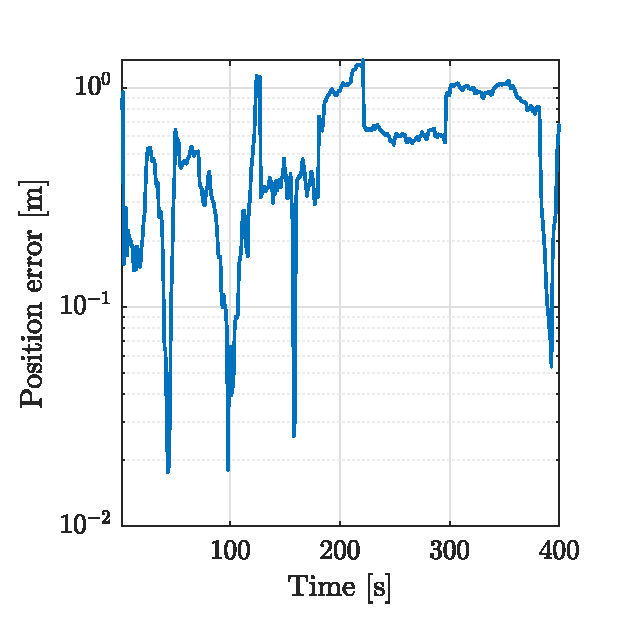
\includegraphics[width = 1\linewidth]{Images/TIRerrorspos.eps}
    \caption{Position AKE}
    \label{fig:TIRerrorspos}
    \end{subfigure}\hfill
    \begin{subfigure}{0.48\linewidth}
    \centering
    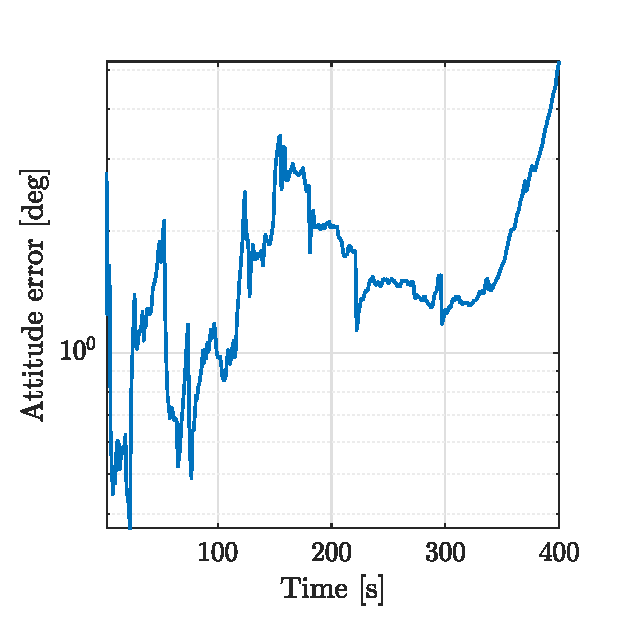
\includegraphics[width = 1\linewidth]{Images/TIRerrorsatt.eps}
    \caption{Attitude AKE}
    \label{fig:TIRerrorsatt}
    \end{subfigure}
    \caption{Position and error for thermal navigation only (hot case)}
    \label{fig:TIRerr_posatt}
\end{figure}

It can be seen that the position estimation provides stable results, while the attitude counterpart consistently presented an error spike at the end of the simulations, suggesting a future divergence of the filter. To characterize the error behavior's source, the Euler angles between the true and estimated target body frame are computed and presented in \cref{fig:anglesZ}, with a rotation sequence Z ($\theta$), Y ($\phi$), X ($\psi$).\\
% As observable in \cref{fig:TIRerrorsatt}, the attitude error spikes significantly by the end of the simulation, suggesting a divergence behavior. Differently from the multispectral or visible case, this result was consistent throughout different simulations, compromising the applicability of thermal-only navigation. To characterize the source of the attitude errors, the Euler angles between the estimated target body frame and the actual target body frame are reported in \cref{fig:anglesZ} according to the sequence of rotation Z ($\theta$), Y ($\phi$), X ($\psi$).\\
% From \cref{fig:anglesZ}, it can be observed that along the whole simulation, and especially at the end, the error accumulates along the z-axis of the target body frame. Being the z-axis the axis of symmetry of VESPA, this drift in the attitude error indicated the arising of symmetry-related issues. Because of the conic shape of VESPA, an accumulation of errors about the x or y target body frame results in an overall change of the shape of the target in the image plane, easily identified and corrected by the tracking algorithm. Regarding the error about the z-axis, the algorithms shall rely on non-symmetric superficial elements such as bolts, flanges, and clamps. If the Image Processing pipeline loses the tracking of these features, it results in a steadily increasing error along the z-axis.
\begin{figure}[!h]
    \centering
    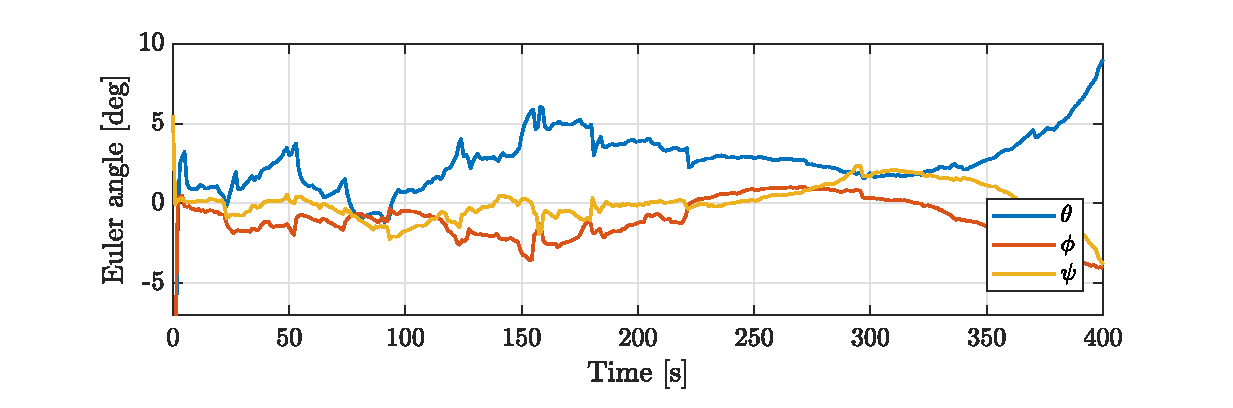
\includegraphics[width = \linewidth]{Images/eulangles_corrected.eps}
    \caption[]{Euler angles between the estimated target body frame and the true target body frame (hot case)}
    \label{fig:anglesZ}
\end{figure}
In \cref{fig:anglesZ}, it can be observed that along the simulation and specifically at the end, the error is mainly concentrated on the z-axis of the VESPA body frame, which is also its axis of symmetry. An error accumulation along this axis indicates that the IP process has difficulties tracking the superficial elements, which, as detailed in \cref{sec:testing}, are the only elements providing information about the relative position about the z-axis of the target. \\
The same consideration could be qualitatively inferred by observing the features tracked by the filter in the first steps of the simulation (\cref{fig:TIRupVespa}) and towards the end (\cref{fig:TIRUpDownVespa}). Both images are subject to CLAHE for contrast enhancement. In the second image, almost no feature is associated with those elements that provide information about the rotation about the axis of symmetry. \\
This effect is due to the low-quality images in terms of resolution and low contrast, which makes it more difficult to detect the beforementioned elements, differently from the visible case. Moreover, to reduce the rendering tool's computational time, the VESPA model has been down-scaled, splitting the conical shape of the target into a limited number of flat surfaces. That creates an apparent contrast gradient on surfaces that otherwise would be textureless. That contrast discontinuity between these regions allows identifying fictitious features which degrade the Image Processing pipeline as they follow a thermal dynamic instead of the rigid body rotational dynamic of the target, favoring an error about the z-axis.\\

\begin{figure}[!h]
    \begin{subfigure}{0.48\linewidth}
    \centering
    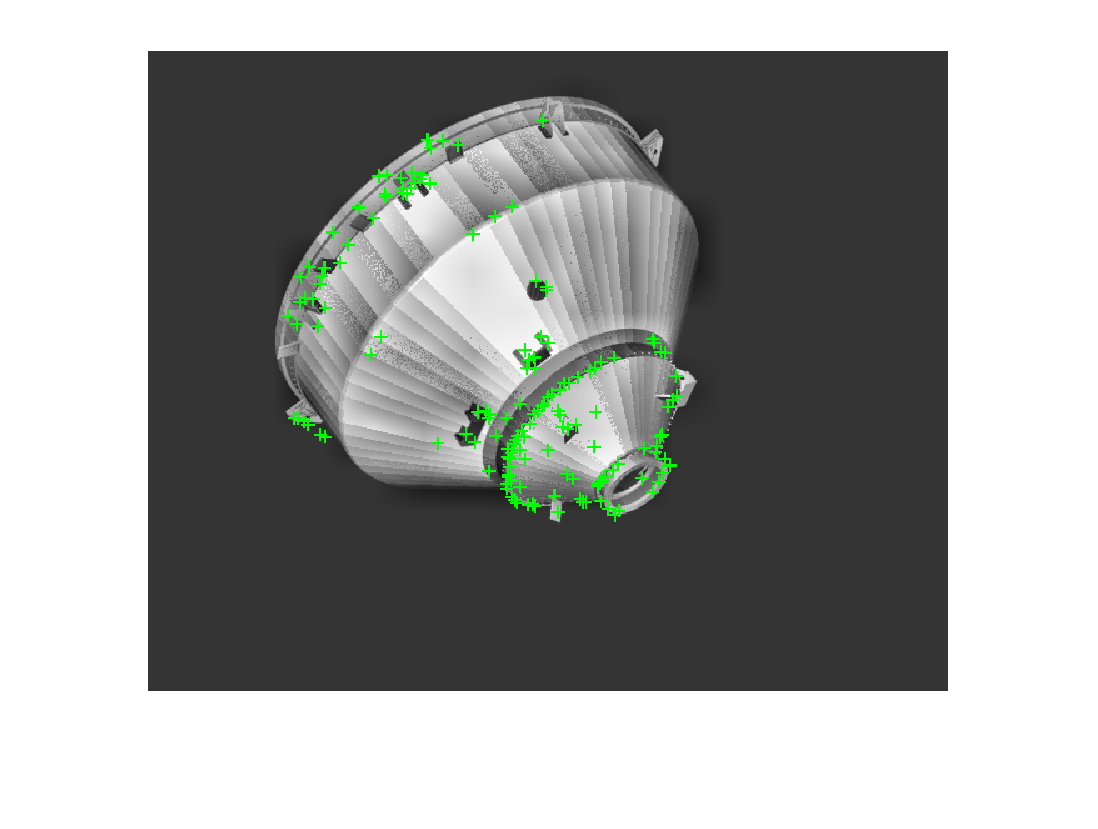
\includegraphics[width = 1\linewidth]{Images/TIRbeginning1.eps}
    \caption{Beginning of the simulation}
    \label{fig:TIRupVespa}
    \end{subfigure}\hfill
    \begin{subfigure}{0.48\linewidth}
    \centering
    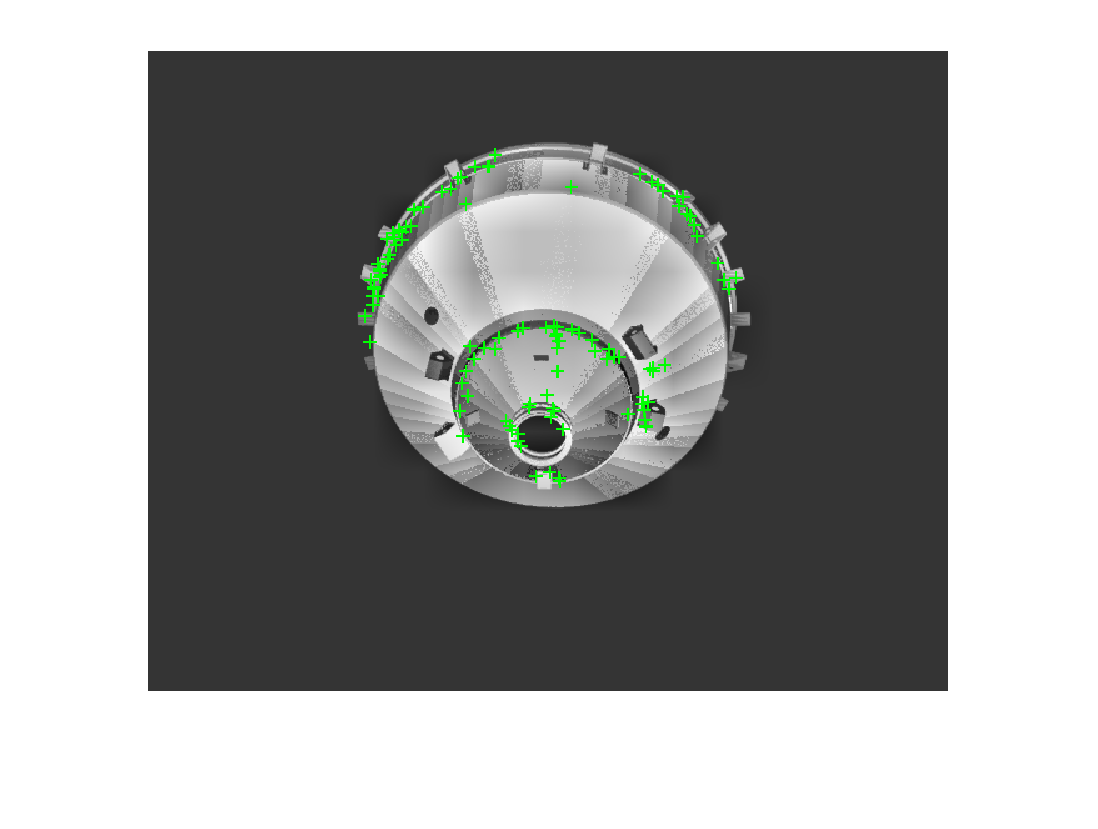
\includegraphics[width = 1\linewidth]{Images/TIRend.eps}
    \caption{End of the simulation}
    \label{fig:TIRDownVespa}
    \end{subfigure}
    \caption{Tracked features on two thermal images of the target}
    \label{fig:TIRUpDownVespa}
\end{figure}

\subsection*{Cold case}
Worse results are obtained during the simulated eclipse, as the image quality is lowered with respect to the presented hot case. The position and attitude error results are reported in \cref{fig:Teclipsr_posatt}. In this case as well, the position estimation works properly, maintaining the error bounded under $\SI{1}{\meter}$. On the contrary, the attitude error presents an almost steadily increasing error, making the estimation diverge.\\
% The obtained results are not satisfactory enough to confirm the viability of thermal navigation as a substitution for the six degrees of freedom visible navigation, lacking the Image Process robustness to be reliable over long periods. However, these results are nevertheless promising, as further development and testing according to the identified shortcomings might solve these issues extending the pipeline range of applicability.

\begin{figure}[!h]
    \begin{subfigure}{0.48\linewidth}
    \centering
    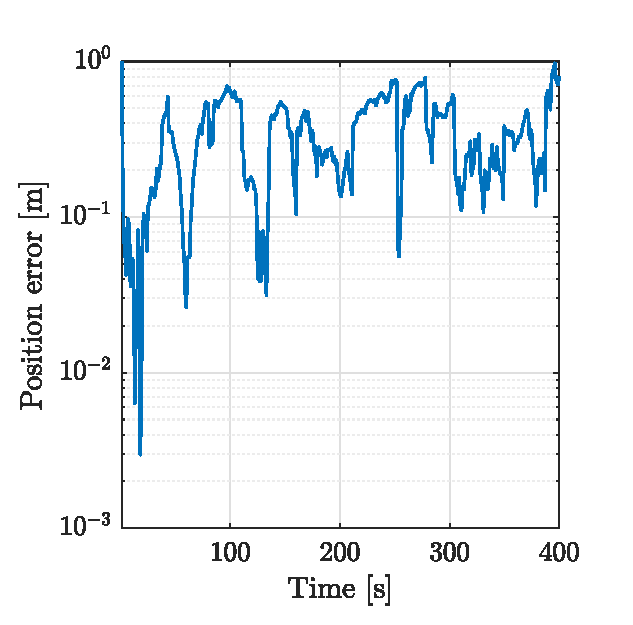
\includegraphics[width = 1\linewidth]{Images/eclipseerrpos.eps}
    \caption{Position AKE}
    \label{fig:eclipsepos}
    \end{subfigure}\hfill
    \begin{subfigure}{0.48\linewidth}
    \centering
    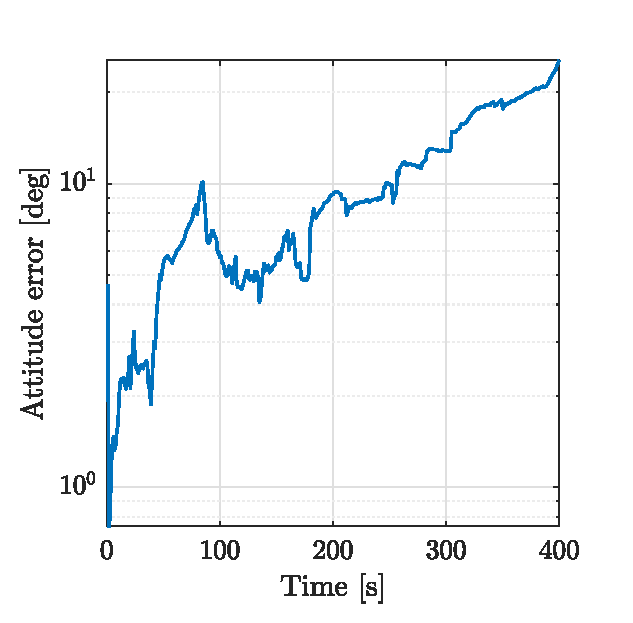
\includegraphics[width = 1\linewidth]{Images/eclipseerratt.eps}
    \caption{Attitude AKE}
    \label{fig:eclispeatt}
    \end{subfigure}
    \caption{Position and attitude errors for thermal navigation only (cold case)}
    \label{fig:Teclipsr_posatt}
\end{figure}
As for the sunlit case, the Euler angles between the estimated and true target body frame are computed and presented in \cref{fig:anglesE}. In this case as well, the drift is unique to the z-axis, but more evident than in the sunlit case because of the lower quality of the image. \\

\begin{figure}[!h]
    \centering
    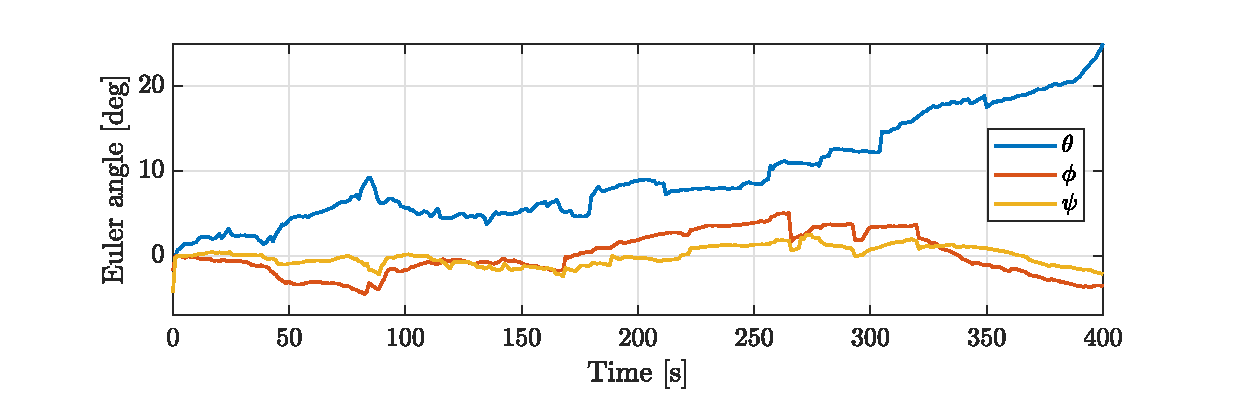
\includegraphics[width = \linewidth]{Images/eulangles_eclipse.eps}
    \caption[Euler angles between the true and estimated target body frame]{Euler angles between the estimated target body frame and the true target body frame (cold case)}
    \label{fig:anglesE}
\end{figure}
As shown in \cref{fig:prepostclahe}, after applying the histogram equalization to the image in eclipse, a good information on the overall target shape is attainable, while the lack of contrast in the image highly compromises the texture; that highly contributes to the error behavior shown in \cref{fig:anglesE}, since an error on the x or y axis produces a significant change of the target shape on the image plane, detectable and correctable by the filter, while an error on the z-axis is hardly observable in terms on Image Processing. 


\begin{figure}[!h]
    \begin{subfigure}{0.48\linewidth}
    \centering
    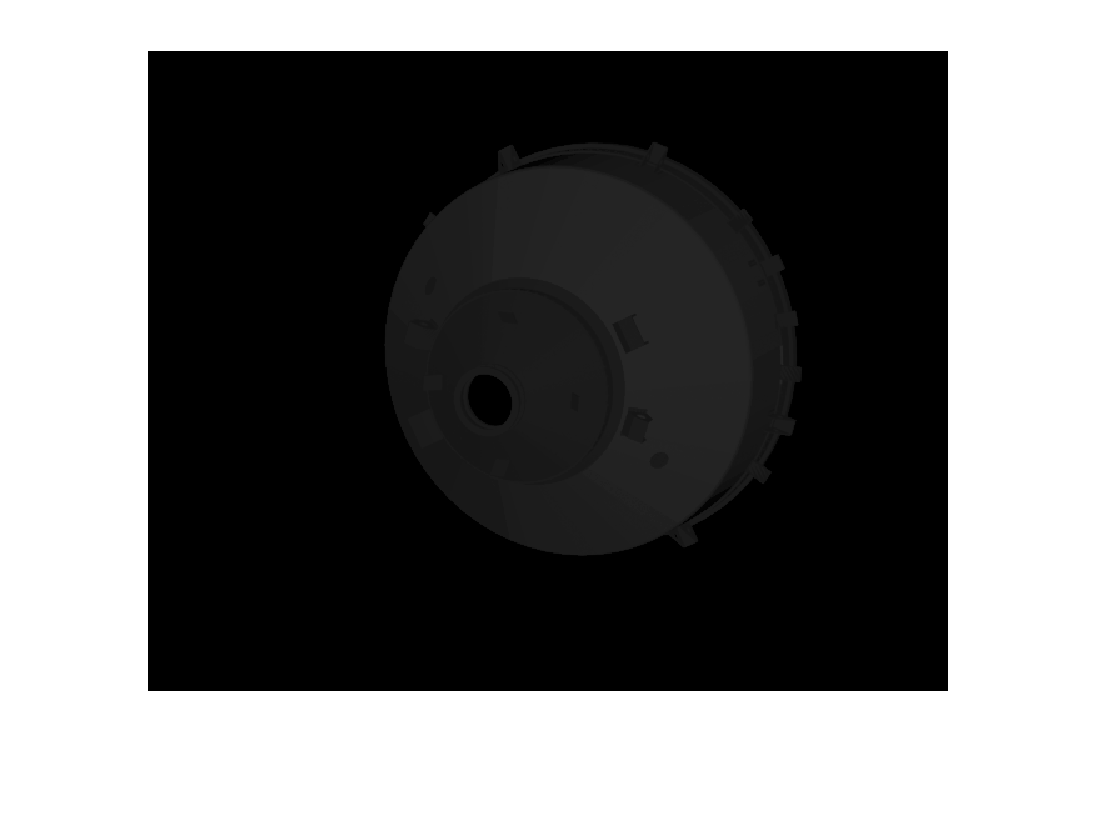
\includegraphics[width = 1\linewidth]{Images/eclipse_preclahe.eps}
    \caption{Raw TIR image in eclipse}
    \label{fig:preclahe}
    \end{subfigure}\hfill
    \begin{subfigure}{0.48\linewidth}
    \centering
    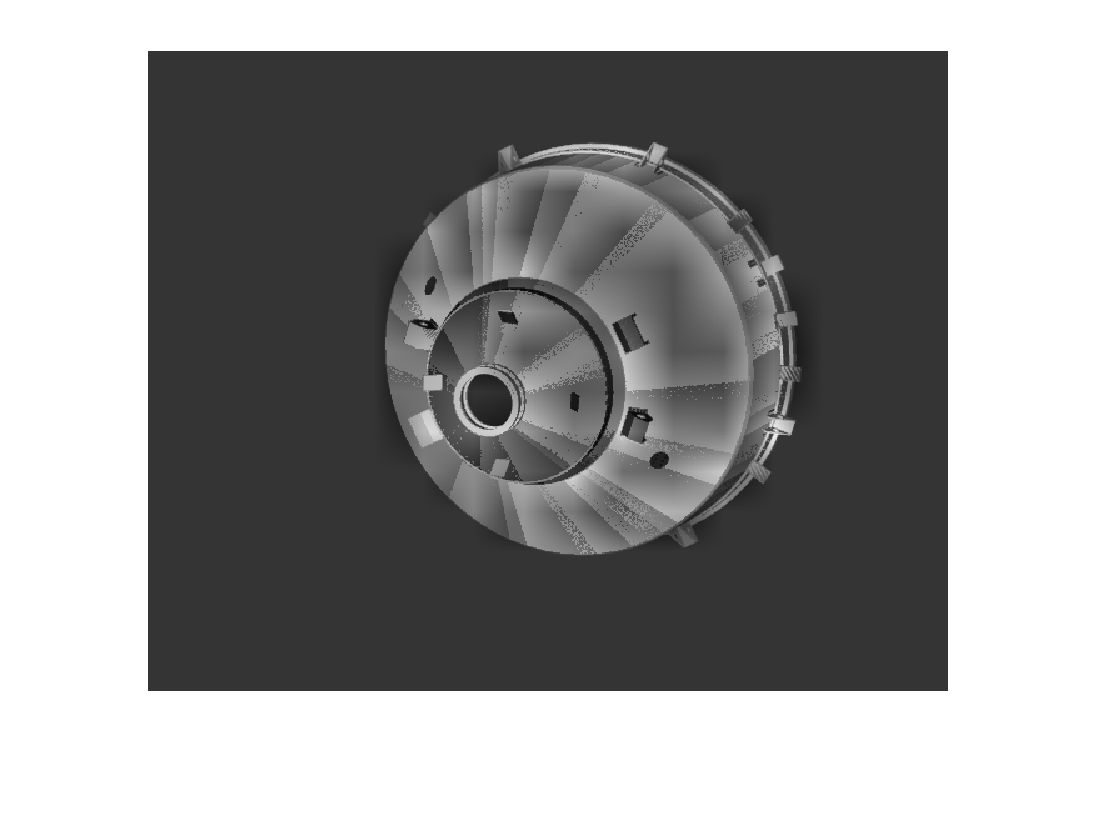
\includegraphics[width = 1\linewidth]{Images/eclipse_postclahe.eps}
    \caption{TIR image in eclipse after CLAHE}
    \label{fig:postclahe}
    \end{subfigure}
    \caption{Original and CLAHE enhanced thermal image in eclipse}
    \label{fig:prepostclahe}
\end{figure}

The obtained results for the sunlit and eclipse case indicate that the proposed navigation filter can not provide reliable standalone pose estimation based on the thermal spectrum only. It shall be noted, however, that most of the criticalities associated with those analyses are related to the symmetrical nature of the target. Further testing on a non-symmetrical target should be performed to test the pipeline in a less critical case, while further work shall be performed to tailor it to apply to symmetrical targets. A possible solution could be to split the IP routine in two segments: one dedicated to the detection of elements that provide information about the relative pose with respect to the x-y axis of the target and one specifically dedicated to the detection of the superficial elements of VESPA for the estimation of the position and attitude about the z-axis (the axis of symmetry). For the former task it would be interesting to extract the ellipses from the images instead of the point features, as suggested in \cite{liu2014relative} for navigation about cylindrical spacecrafts.\\
Finally, the validity of the results proposed is limited by the strong assumptions made on the thermal model of the target. A more refined thermal model should be introduced to further characterize the navigation pipeline to consider aspects such as non-uniform thermal profiles. 


\subsection{Test 4: Target-chaser distance dependability }
The visual navigation filter scope is to enhance close proximity navigation capabilities. It is, therefore, necessary to identify the limit of application in terms of distance from the target for which the proposed solution can be used. \\
Different simulations have been performed on images rendered considering an increasing distance from the target. Because of the time required for image rendering, only four sets of 100 VIS and TIR images have been generated, considering an average distance of $\SI{20}{\meter}$, $\SI{40}{\meter}$, $\SI{50}{\meter}$, and $\SI{80}{\meter}$. Those distances were selected to range from a condition where the target fully occupies the image up to critical distance where the superficial features are hardly identifiable (\cref{fig:VISdistance}). The simulation at different distances have been performed with the same illumination conditions, reported in \cref{tab:contest4}, to enable a meaningful comparison of the results.\\
Sample images at different distances are reported in \cref{fig:VISdistance,fig:TIRdistance}.\\

\begin{table}[!h]
    \centering
    \begin{tabular}{ C{1.8cm} C{1.8cm} C{5cm}}
      $\phi$ & $\rho$ & Relative distance\\ \hline\hline
      $\SI{25}{\deg}$ & $>\SI{0}{\deg}$ & $[\SI{20}{\meter}, \SI{40}{\meter}, \SI{50}{\meter}, \SI{80}{\meter}]$\\\hline
   
    \end{tabular}
    \caption{Test 4 illumination conditions and relative distances}
    \label{tab:contest4}
\end{table}


\begin{figure}[!h]
    \begin{subfigure}{0.24\linewidth}
        \centering
        \includegraphics[width=\linewidth]{Images/VIS10m.png}
    \end{subfigure}\hfill
    \begin{subfigure}{0.24\linewidth}
        \centering
        \includegraphics[width=\linewidth]{Images/VIS20m.png}
    \end{subfigure}\hfill
    \begin{subfigure}{0.24\linewidth}
        \centering
        \includegraphics[width=\linewidth]{Images/VIS50m.png}
    \end{subfigure}\hfill
    \begin{subfigure}{0.24\linewidth}
        \centering
        \includegraphics[width=\linewidth]{Images/VIS80m.png}
    \end{subfigure}
    \caption[Visible images rendered at different distances]{Visible images rendered at different distances: $\SI{20}{\meter}$ (leftmost), $\SI{40}{\meter}$ (left), $\SI{50}{\meter}$ (right), $\SI{80}{\meter}$ (rightmost)}
    \label{fig:VISdistance}
\end{figure}
\begin{figure}[!h]
    \begin{subfigure}{0.24\linewidth}
        \centering
        \includegraphics[width=\linewidth]{Images/TIR20m.png}
    \end{subfigure}\hfill
    \begin{subfigure}{0.24\linewidth}
        \centering
        \includegraphics[width=\linewidth]{Images/TIR40m.png}
    \end{subfigure}\hfill
    \begin{subfigure}{0.24\linewidth}
        \centering
        \includegraphics[width=\linewidth]{Images/TIR50m.png}
    \end{subfigure}\hfill
    \begin{subfigure}{0.24\linewidth}
        \centering
        \includegraphics[width=\linewidth]{Images/TIR80m.png}
    \end{subfigure}
    \caption[Thermal images rendered at different distances]{Thermal images rendered at different distances: $\SI{20}{\meter}$ (leftmost), $\SI{40}{\meter}$ (left), $\SI{50}{\meter}$ (right), $\SI{80}{\meter}$ (rightmost)}
    \label{fig:TIRdistance}
\end{figure}
The position Relative MKE and attitude Absolute MKE over a run performed for each distance is reported in \cref{fig:disterrors}.  The numerical results with the associated standard deviation are also reported in \cref{tab:Disterrors}. As expected, there is a steady increase in both the parameters estimated by the filter under equal values of $\phi$ and $\rho$, as the information provided by the images decreases with the distance.\\

\begin{figure}[!h]
    \begin{subfigure}{0.48\linewidth}
        \centering
        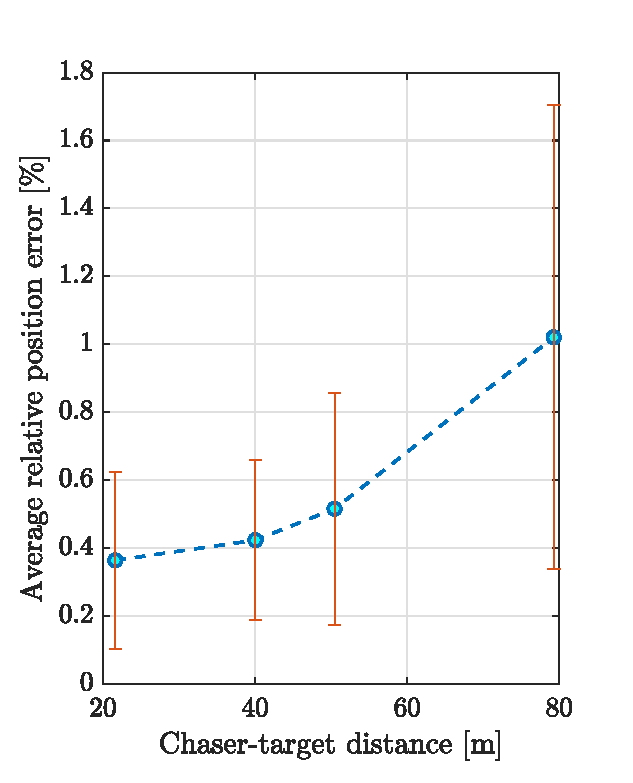
\includegraphics[width=\linewidth]{Images/DistPos.eps}
    \end{subfigure}\hfill
    \begin{subfigure}{0.48\linewidth}
        \centering
        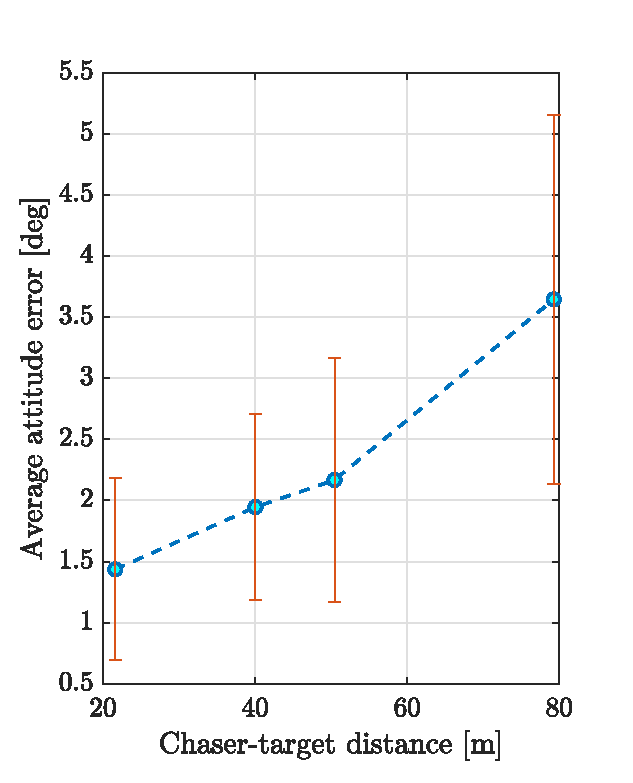
\includegraphics[width=\linewidth]{Images/DistAtt.eps}
    \end{subfigure}
    \caption[Average position and attitude errors at different distances]{Position relative MKE (left) and attitude absolute MKE (right) errors along different simulations with associated standard deviation}
    \label{fig:disterrors}
\end{figure}

\begin{table}[h]
    \begin{subtable}[h]{1\textwidth}
        \centering
        \begin{tabular}{l  c c}
        Distance & Absolute MKE [$\SI{}{\meter}$]& Relative MKE [\%]\\ \hline \hline
        $\SI{20}{\meter}$ & $0.07\pm 0.05$ & $0.37\pm 0.26$\\\hline
        $\SI{40}{\meter}$ & $0.17\pm 0.10$ & $0.42\pm 0.24$\\\hline
        $\SI{50}{\meter}$ & $0.28\pm 0.17$ & $0.52\pm 0.34$\\\hline
        $\SI{80}{\meter}$ & $0.82\pm 0.55$ & $1.02\pm 0.68$\\\hline
        
       \end{tabular}
       \caption{Position errors}
       \label{tab:distpos}
    \end{subtable}
    \hfill
    \begin{subtable}[h]{1\textwidth}
        \centering
        \begin{tabular}{l  c }
        Distance & Absolute MKE [$\SI{}{\deg}$]\\ \hline \hline
        $\SI{20}{\meter}$ &  $1.44\pm 0.72$ \\\hline
        $\SI{40}{\meter}$ &  $1.94\pm 0.76$ \\\hline
        $\SI{50}{\meter}$ &  $2.16\pm 1.00$ \\\hline
        $\SI{80}{\meter}$ &  $3.64\pm 1.50$ \\\hline
        \end{tabular}
        \caption{Attitude errors}
        \label{tab:distatt}
     \end{subtable}
     \caption{Position and attitude errors at different chaser-target distances}
     \label{tab:Disterrors}
\end{table}
\mbox{}\\
\cref{fig:disterrors,tab:Disterrors} show that with the distance, there is also an increase in the standard deviation of the error. This derives from a high fluctuation in the error values that could bring instabilities in more extended simulations. 
This performance degradation is attributable to the Image Processing pipeline, as the lower dimension of the target in the image plane compromises the feature detection and matching.\\
Given the presented results and the cameras' parameters used to render the images, the proposed pipeline is suitable for the close-range inspection and final approach phases, limiting the chaser-target distance to $\SI{50}{\meter}$. To extend the application range, possible solutions include different navigation techniques such as angles-only navigation, either avoiding a 6-DoF pose reconstruction, or including in the sensor suite cameras with different FOVs to provide higher quality images at higher distances.


\subsection{Test 5: synchronous rotation }
A final analysis was carried out investigating the capability of the filter to work correctly in the case there is synchronous rotation between the chaser and the target, giving the appearance that there is no relative motion between the two. This situation is tested in favorable condition for both spectra. The chaser-target distance and the illumination parameters are reported in \cref{tab:contest5}.

\begin{table}[!h]
    \centering
    \begin{tabular}{ C{1.8cm} C{1.8cm} C{5cm}}
      $\phi$ & $\rho$ & Relative distance\\ \hline\hline
      $\SI{25}{\deg}$ & $\approx\SI{0}{\deg}$ & $\SI{35}{\meter}$\\\hline
   
    \end{tabular}
    \caption{Test 5 illumination conditions and relative distance}
    \label{tab:contest5}
\end{table}

As detailed in the results analysis, two simulations have been performed with the same environmental conditions (\cref{tab:contest5}), initial conditions and tuning of the filter to highlight the non-deterministic behavior of the navigation filter. \\
The chaser trajectory in the target body frame can be observed in \cref{fig:synchtraj}. As expected it is almost point-like. This is obtained by setting the angular velocity of the target equal to the opposite of the angular velocity of the chaser position about the target. All other angular velocities are set to zero.\\

\begin{figure}[!h]
    \centering
    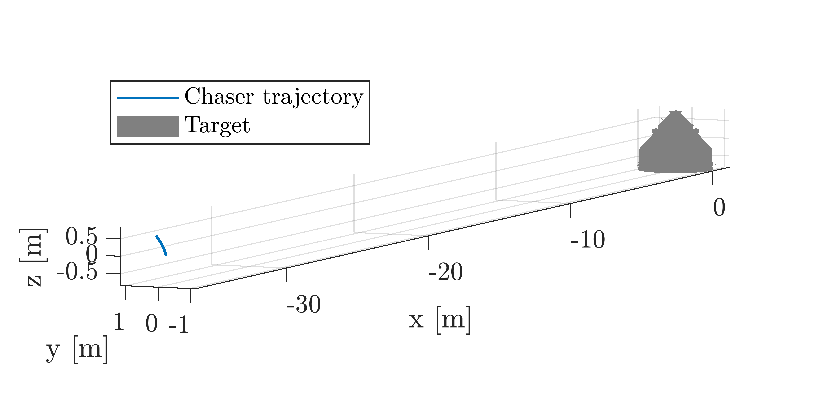
\includegraphics[clip,trim = 0cm 0cm 0cm 0cm,width = 0.6\linewidth]{Images/synchtraj.eps}
    \caption[Trajectory in case of quasi-synchronous rotation]{Chaser trajectory in the target body frame in the case of quasi-synchronous motion}
    \label{fig:synchtraj}
\end{figure}
%%The results for two different simulations are reported in \cref{fig:syncherrors} for two different simulations.

%The synchronicity resulted to be a favourable condition for the proposed navigation pipeline, as the stress on the Image Processing routine is minimal.
%The results for two simulations performed in the same conditions are reported in \cref{fig:syncherrors} for two different simulations. 
%In both cases, the filters present no problems in estimating the attitude and position of the target. Because of the attitude-position dynamical coupling, the apparent stasis of the features on the image plane is recognised as the synchronous of the target with the relative position of chaser. \\
%This is because of the attitude-position dynamical coupling, as it allows the filter to consider the chaser's motion and orientation with respect to the target, even in cases where there appears to be no relative motion between the two.\\
%It can be observed that the error behavior is more stable than in the results reported in the previous analysis. This is because the IP pipeline is working in optimal conditions, as there is a very mild flow of the features, enhancing the tracking performance, and there is no feature loss over time. However, as highlighted by the behavior of the two simulations, the results strongly rely on the quality of the first feature initialization, which has partially randomic performances because of the initial error and the RANSAC routine. As there is no loss of features over time, if the first initialization contains a high percentage of outliers or a bias, these errors are maintained over time.\\


\begin{figure}[!h]
    \begin{subfigure}{0.48\linewidth}
        \centering
        \includegraphics[width = \linewidth]{Images/synchpos.eps}
        \caption{Position AKE}
    \end{subfigure}\hfill
    \begin{subfigure}{0.48\linewidth}
        \centering
        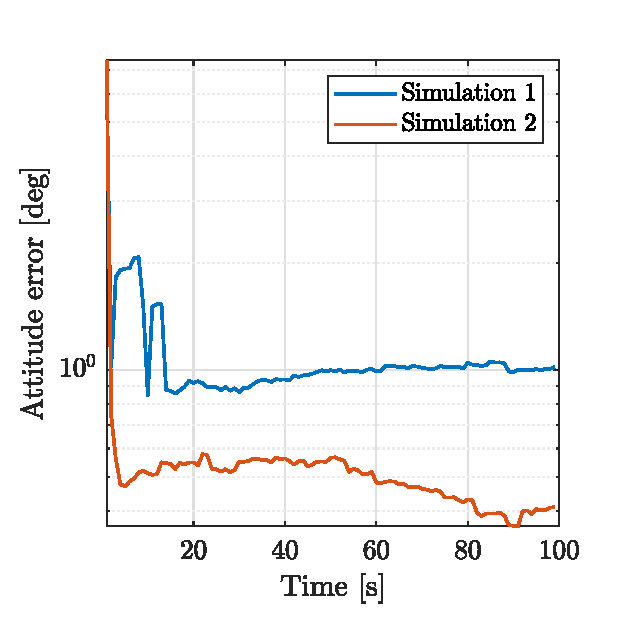
\includegraphics[width = \linewidth]{Images/synchatt.eps}
        \caption{Attitude AKE}
    \end{subfigure}
    \caption[Position and attitude errors in the case of quasi-synchronous motion]{Position and attitude errors for two simulations in the case of quasi-synchronous motion}
    \label{fig:syncherrors}
\end{figure}

In \cref{fig:syncherrors} the error behavior along the two simulations performed can be observed. The two simulations have been executed with an identical initialization of the parameters and environmental conditions; the difference in the results is justified only by the non-deterministic behavior of the navigation chain. In both cases, the filters present no problems in estimating the attitude and position of the target. Because of the attitude-position dynamical coupling, the apparent stasis of the features on the image plane is recognized as the synchronous rotation of the target with the relative position of chaser. \\
 In the case of synchronous rotation, the features are quasi-static on the image plane, requiring for no feature re-initialization as there is no feature loss. This aspect has two main effects: primarily, it increases the filter's performances relaxing the tracking step, resulting in a more stable estimation. Secondly, the filter's performances are mostly influenced by the quality of the first matching between the image points and the model landmarks, which is affected by randomic aspects such as the RANSAC routine. If the association presents an increased number of outliers, the navigation will be consistently affected by an increased error (Simulation 1), while if it provides good feature associations, the errors are lowered (Simulation 2).\\
From the results presented, the synchronous motion does not represent a critical condition for the proposed navigation pipeline. On the contrary, because of the null relative angular rates, it represents a favorable condition facilitating the IP process.

\section{Final remarks}
\chaptermark{Numerical Simulations}
The results obtained on the test plan provide an insightful overview of the proposed navigation chain performances and limitations. The key findings for each test case are reported in \cref{tab:finalrem} to provide a concise yet exhaustive summary of the obtained results. 

%\begin{table}[H]
%\centering
\begin{longtable}{l p{2.5cm} p{11.5cm}}

Test n. & Illumination & Final remarks\\ \lline{3}
1 & Case A & Whenever the target is well illuminated and clearly visible both in the VIS and TIR image, the proposed navigation chain can reliably estimate the 6-DoF relative pose. In this condition the fusion of the VIS \& TIR information enhances the results, highlighting the positive contribution of sensor fusion. Those results suggest that a tightly coupled filtering approach is suitable for multispectral relative navigation applications. The main limitation identified in this condition is the elevated computational time required for the re-initialization step, which exceeds the filter's update frequency.\\\hline
%However, the algorithm overestimates the uncertainty of the relative velocity and angular rates, indicating the need for a more accurate dynamic or a better tuning of the filter parameters. Moreover, the computational time of the re-initialization step exceeds the update frequency of the filter, requiring further work aimed at the reduction of the run time of this process.  \\ \hline
2 & Cases B,C & The multispectral navigation chain fails if the VIS image is compromised by low illumination conditions, indicating that the visible spectrum is the mainstay of the algorithm's robustness. The phase angle $\phi$ and the elevation angle $\rho$ resulted to be equally influential on the navigation pipeline performances, restraining the algorithm's application to a limited range of environmental conditions. As the VIS contribution is counterproductive in low illumination conditions, the solution identified is to discard the visible information when this condition arises. \\ \hline
3 & Cases B,D & Thermal navigation could not provide reliable pose estimate in both the hot case (Case B) and cold case (Case D). In both cases the navigation chain fails to estimate the relative position about the axis of symmetry of VESPA, resulting in a diverging attitude estimation. The cause of this behavior is identified in the lower performances of the IP routine applied to TIR images, which is not able to track the superficial elements of the target.  \\ \hline
4 & Case A & The navigation performances are highly influenced by the the chaser-target distance. With the considered camera proprieties it is evaluated that the the proposed application is suited for CPO under a relative distance of 50 m, as it does not provide reliable results if the chaser and the target are further apart.\\ \hline
5 & Case A & The navigation chain works properly also under a synchronous motion condition. The dynamical and measurement models enable the filter to estimate all the states correctly also in this peculiar relative motion. Moreover, the performances are improved as the quasi static appearance of the target on the image plane relaxes the IP routine.  \\ \hline
\caption{Final remarks for each test case and illumination condition}
\label{tab:finalrem}
\end{longtable}
% To conclude, the correct operation of the algorithm in nominal case and the contribution of imaging sensor fusion (Test 1) highlights that the work done lays an interested foundation for future research in multispectral navigation. The poor results obtained in terms of robustness to illumination conditions (Tests 2,3) identify the thermal navigation as the limiting aspect of the proposed research.
%\end{table}

\section{Image fusion comparative assessment}
\chaptermark{Numerical Simulations}
In this section, a comparative assessment of the proposed pipeline is performed with respect to the obtained results by \cite{piccinin2023spacecraft} regarding multispectral relative navigation performing sensor fusion at image level. The reference work and the thesis investigate the multispectral navigation problem in two very different situations, as one performs pose estimation about a small body while the other is applied to artificial space objects. Moreover, the asteroid navigation is performed with a SLAM approach, as the target is not initially known, while the thesis work proposes a model-based solution to the navigation problem. Finally, it shall be noted that the analyses performed in \cite{piccinin2023spacecraft} are performed with a more realistic testing framework, providing a more reliable insight on the subject. These important differences limit to a qualitative comparison only.\\
Both methods perform well in good illumination conditions, solving the pose throughout the simulations. For the image fusion technique, it is found that, in nominal conditions, it performs slightly worse than using visible-only or thermal-only images. This is not the case for the proposed pipeline, where the sensor fusion enhances navigation performances. This is due to the introduction of noise in the image fusion process, avoided in the navigation filter. On the other hand, image fusion enables stronger reliability in cases where the target is only partially visible in the VIS image. While the visible contribution in the proposed filter becomes counterproductive, in the image fusion technique, this does not happen, enabling wider multispectral navigation applicability. Finally, in low illumination conditions, both methods are unreliable, showing invalid results.\\
The consistency of the results in the two applications highlights the need for more maturity of multispectral navigation in scarce illumination conditions, where the thermal sensor should increase the range of applicability. The proposed sensor fusion method outperforms the image-fusion technique when the target is well visible in both the VIS and TIR images. However, the latter is more robust when the visible image is less performing. To the best of the author's knowledge, both methods take advantage of a switch between different modalities based on real-time environmental conditions. \\
A schematic of the comparison between the proposed filter-based multispectral navigation pipeline and the image fusion-based one proposed in \cite{piccinin2023spacecraft} is reported in \cref{tab:compa}.

\begin{table}[!h]
    \centering
    \begin{tabular}{l p{6cm} p{6cm}}
         & Filter-based & Image fusion \\\hline\hline
       low $\phi$  & Reliable pose estimation; VIS \& TIR fusion provide the best solution & Reliable pose estimation; VIS only provides the best results \\\hline 
       high $\phi$  & Unreliable pose estimation & Reliable pose estimation; VIS \& TIR fusion provides the best results \\\hline 
       eclipse/shadow  & Unreliable pose estimation & Unreliable pose estimation \\\hline 
    \end{tabular}
    \caption{Comparison between the presented filter-based multispectral navigation pipeline and the image fusion based proposed in \cite{piccinin2023spacecraft}}
    \label{tab:compa}
\end{table}
Based on the comparison presented in \cref{tab:compa}, it appears that image fusion is more advantageous than the method proposed in the thesis because it is more resistant to low illumination of the target. However, due to the significant differences between the two applications and the respective synthetic images, it is not possible to definitively determine which method is superior. To answer the question of whether there is a winner between tightly, loosely, and image-fusion based approaches, it is necessary to apply them to the same test case to have quantitatively comparable results.

% \lettrine{T}{he} numerical simulation's results are presented in the present chapter. Firstly, a general overview of filter performances in a nominal situation is performed. As during the test of the proposed pipeline different shortcomings have been identified, this first analysis is performed in a situation that avoids these criticalities, enabling to present the algorithm's performances in a nominal situation.
% Subsequently, the limitations identified are presented ad discussed. To achieve this, the algorithm have been stressed to highlight its dependency on the illumination conditions, the scarce performances given by TIR-only navigation, and the dependability on the chaser-target distance. The review of the applicability of the proposed navigation pipeline sets the basis for the final remarks and suggestions for future works.

% \section{Nominal performances}
% \chaptermark{Numerical Simulations}

% As the pose initialization has not been performed in thesis work, for the initialization filter a initial error based on the results of \cite{pesce2019autonomous} was applied to the ground truth. For the position, randomly generated error between $\SI{0}{\meter}$ and $\SI{1}{\meter}$ was applied to each of the components, while the true initial attitude is rotated of five degrees about a random vector. As the pose initialization provides no information on the relative velocity or angular rates, those are set to zero at the first step of the filter.\\
% The process noise covariance was defined as a diagonal matrix. The values used to build the matrix are reported in \cref{tab:Q0} and have been computed with a trial and error procedure. It shall be noted that over result is not sensible to small variations of these values. For what regards the initialization of the covariance matrix $\vect{P}$, to take into account the important initial errors overestimated values have been assigned to its diagonal elements, as observable from \cref{tab:P0}. This reflects the initial uncertainty given by the pose acquisition and enables the filter to converge to its steady-state performances.\\
% \begin{table}[h]
%     \begin{subtable}[h]{0.45\textwidth}
%         \centering
%         \begin{tabular}{l  c c}
%         Parameter & Value & Unit\\ \hline \hline
%         $\sigma_{\vect{x}}^2 $ & $\expnumber{2.3}{+0}$ & \SI{}{\meter^2}\\\hline
%         $\sigma_{\dot{\vect{x}}}^2 $ & $\expnumber{2.0}{-3}$ & \SI{}{\meter^2\per\second^2}\\\hline
%         $\sigma_{\vect{a}_p}^2 $ & $\expnumber{4.0}{-2}$ & /\\\hline
%         $\sigma_{\omega}^2 $ & $\expnumber{2.5}{-3}$ & \SI{}{\radian^2\per\second^2}\\\hline
        
%        \end{tabular}
%        \caption{Process noise covariance diagonal elements}
%        \label{tab:Q0}
%     \end{subtable}
%     \hfill
%     \begin{subtable}[h]{0.45\textwidth}
%         \centering
%         \begin{tabular}{l  c c}
%         Parameter & Value & Unit\\ \hline \hline
%         $\sigma_{\vect{x}}^2 $ & $\expnumber{1.0}{+0}$ & \SI{}{\meter^2}\\\hline
%         $\sigma_{\dot{\vect{x}}}^2 $ & $\expnumber{8.0}{-2}$ & \SI{}{\meter^2\per\second^2}\\\hline
%         $\sigma_{\vect{a}_p}^2 $ & $\expnumber{1.0}{-2}$ & /\\\hline
%         $\sigma_{\omega}^2 $ & $\expnumber{2.0}{-1}$ & \SI{}{\radian^2\per\second^2}\\\hline
%         \end{tabular}
%         \caption{Initial covariance matrix settings}
%         \label{tab:P0}
%      \end{subtable}
%      \caption{Diagonal values of the matrices $\vect{Q}$ and $\vect{P}$ at the initial step of the filter}
%      \label{tab:PQinit}
% \end{table}
% The filter initialization also requires to provide an initial value for the measurement covariance matrix. The values within this matrix are then corrected at each step of the filter, but providing an initial guess to far from the estimated values might cause numerical errors at the features re-initialization steps. For this reason, the values assigned have been selected by considering the filter estimations. The standard deviation used to compute the matrix is reported in \cref{tab:R0}. The measurement noise matrix will result is a square-diagonal matrix with dimension twice the number of features in the model. At each step the matrix is pruned of the elements that refers to features not associated to an image point. From \cref{tab:R0} and the dimension of the images, it is possible to estimate that the noise associated with the visible features is about half the one associated with the thermal features.  The criteria used to initialize these values was to consider the average value that the filter estimated during saple runs. 
% \begin{table}[!h]
%     \centering
%         \begin{tabular}{l  c c}
%         Parameter & Value & Unit\\ \hline \hline
%         $\sigma_{VIS} $ & $14$ & \SI{}{\pixel}\\\hline
%         $\sigma_{TIR} $ & $7$ & \SI{}{\pixel}\\\hline
%         \end{tabular}
%         \caption{Initial standard deviation assigned to the features}
%     \label{tab:R0}
% \end{table}
% The parameters reported in \cref{tab:PQinit,tab:R0} are used the the performance analysis reported in the following section. For further analysis regarding the applicability of the proposed pipeline these parameters have been further tuned to try to adapt the application to different situations.


% \newpage
% \section{Performance analysis}
% \chaptermark{Numerical Simulations}
% The nominal performances of the algorithm are presented testing it on a 400-images database rendered with the target maintaining an average distance of $\SI{40}{\meter}$ from the target. The trajectory of the chaser in the target LVLH and body frame is reported in \cref{fig:trajbody,fig:trajLVLH}. The visible and thermal images have been generated with the chaser-target-Sun angle of $\SI{25}{\deg}$. This condition provides a good illumination of the target without causing artifacts such as reflections or significant shadows that, as explain later, represent an important limitation for the visible image processing routine. \\
% \begin{figure}[!h]
%     \begin{subfigure}[b]{0.48\textwidth}
%     \centering
%     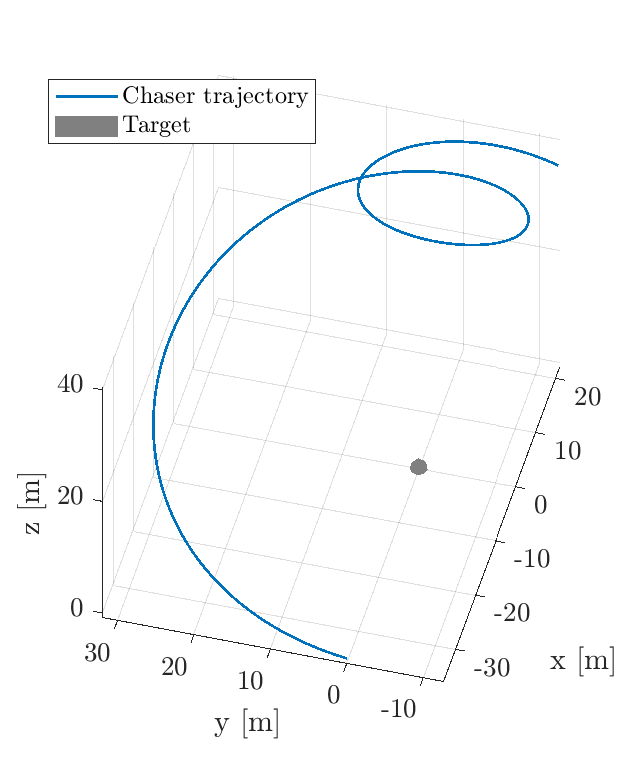
\includegraphics[clip,trim = 0cm 0cm 0cm 1cm,width=\linewidth]{Images/bodyttraj.eps}
%     \caption{Target body frame}
%     \label{fig:trajbody}
%     \end{subfigure}\hfill
%     \begin{subfigure}[b]{0.48\textwidth}
%     \centering
%     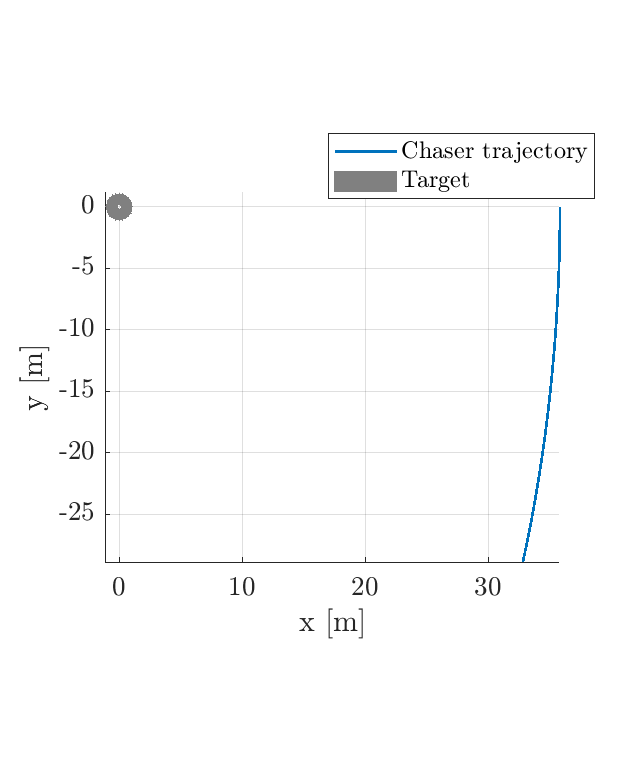
\includegraphics[clip,trim = 0cm 2cm 0cm 1cm,width=\linewidth]{Images/lvlhttaj.eps}
%     \caption{Target LVLH frame}
%     \label{fig:trajLVLH}
%     \end{subfigure}
%     \caption{Chaser trajectory in target's body frame and LVLH frame}
%     \label{fig:trak}
% \end{figure}

% On this trajectory the navigation algorithm have been used testing both the VIS-TIR fusion, as well as visible-only and thermal-only navigation. The results in terms of position and attitude errors, according to the definition \mycomm{add reference}, are presented in \cref{fig:err_posatt}.\\
% A first positive result that can be deduced by the error behaviour is that the algorithm is stable along the simulations, as both the position and attitude error remains bounded for the multispectral case. Moreover, the algorithm presents a fast transient behaviour recovering with just a few filter steps the initial error given by the initialization. 
% \begin{figure}[!h]
%     \begin{subfigure}[b]{1\textwidth}
%     \centering
%     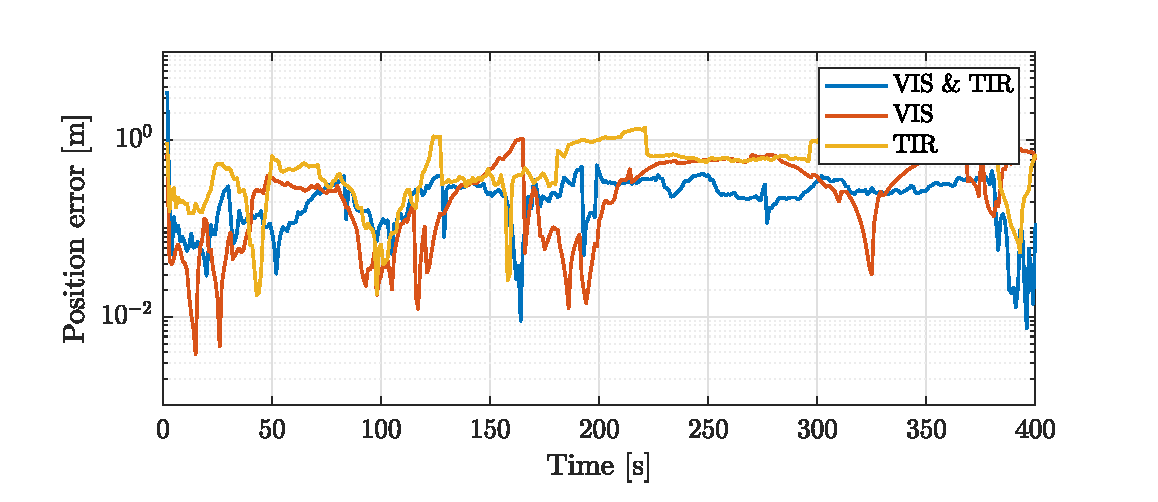
\includegraphics[width=0.93\linewidth]{Images/err_pos.eps}
%     \caption{Position errors}
%     \label{fig:err_pos}
%     \end{subfigure}\hfill
%     \begin{subfigure}[b]{1\textwidth}
%     \centering
%     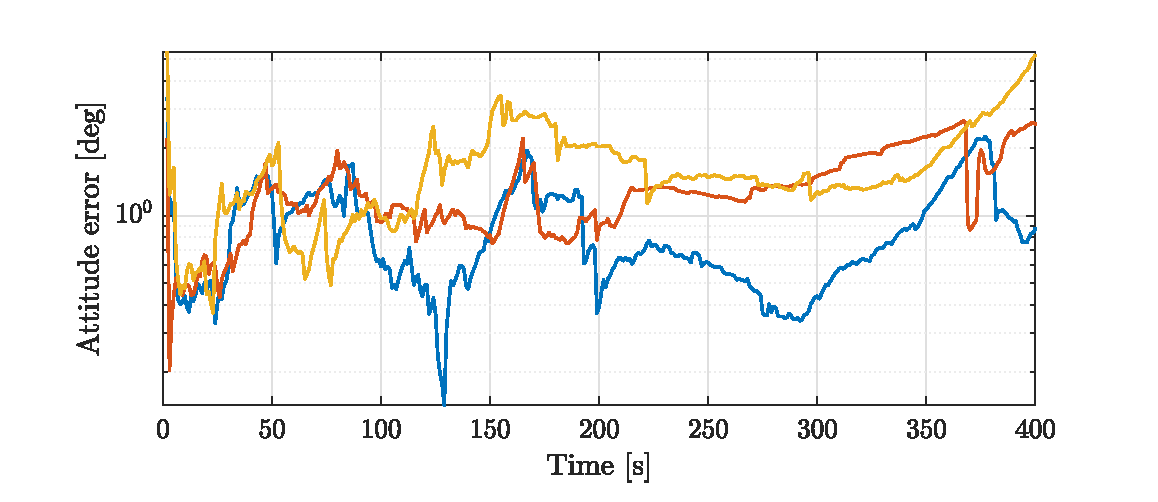
\includegraphics[width=0.93\linewidth]{Images/err_att.eps}
%     \caption{Attitude errors}
%     \label{fig:err_att}
%     \end{subfigure}
%     \caption{Chaser trajectory in target's body frame and LVLH frame}
%     \label{fig:err_posatt}
% \end{figure}
% \begin{table}[!h]
%     \begin{subtable}[h]{0.55\textwidth}
%         \centering
%         \begin{tabular}{l  c c}
%         Spectrum & Absolute error [$\SI{}{\meter}$]& Relative error\\ \hline \hline
%         VIS \& TIR &$0.25\pm 0.54$ & $0.63\pm 0.54$\\\hline
%         VIS & $0.35\pm 0.59$ & $0.85\pm 0.60$\\\hline
%         TIR & $0.59\pm 0.81$ & $1.51\pm 0.82$\\\hline
        
%        \end{tabular}
%        \caption{Position errors}
%        \label{tab:poserrs}
%     \end{subtable}
%     \hfill
%     \begin{subtable}[h]{0.42\textwidth}
%         \centering
%         \begin{tabular}{l  c }
%         Spectrum & Absolute error [$\SI{}{\deg}$]\\ \hline \hline
%         VIS \& TIR &  $0.86\pm 0.44$\\\hline
%         VIS &  $1.32\pm 0.52$ \\\hline
%         TIR &  $1.68\pm 0.83$ \\\hline
%         \end{tabular}
%         \caption{Attitude errors}
%         \label{tab:atterrs}
%      \end{subtable}
%      \caption{Position and attitude errors for the different spectrum modalities}
%      \label{tab:posatters}
% \end{table}
% From these plots it is possible to qualitatively observe how the fusion of the visible and thermal spectra presents an improvement as it reduces the errors and improve the stability of the estimation process. As expected from the low quality of the data provided, the thermal camera perform worse than the fused sensors and the visible camera alone. 
% For a more quantitative analysis of the results the average error and the associated standard deviation is computed and reported in \cref{tab:posatters}, confirming want inferred from the \cref{fig:err_pos,fig:err_att}. \\
% Given the errors absolute and relative values, it is possible to conclude that these results are suitable for the relative navigation application. The same consideration can be inferred by observing the estimated position of the chaser in the target body frame \cref{fig:esttraj}, which is affected both from the attitude and the position errors. After correcting the initial error, the trajectory is followed truthfully, making the estimation suitable for applications such as ADR. 
% \begin{figure}
%     \centering
%     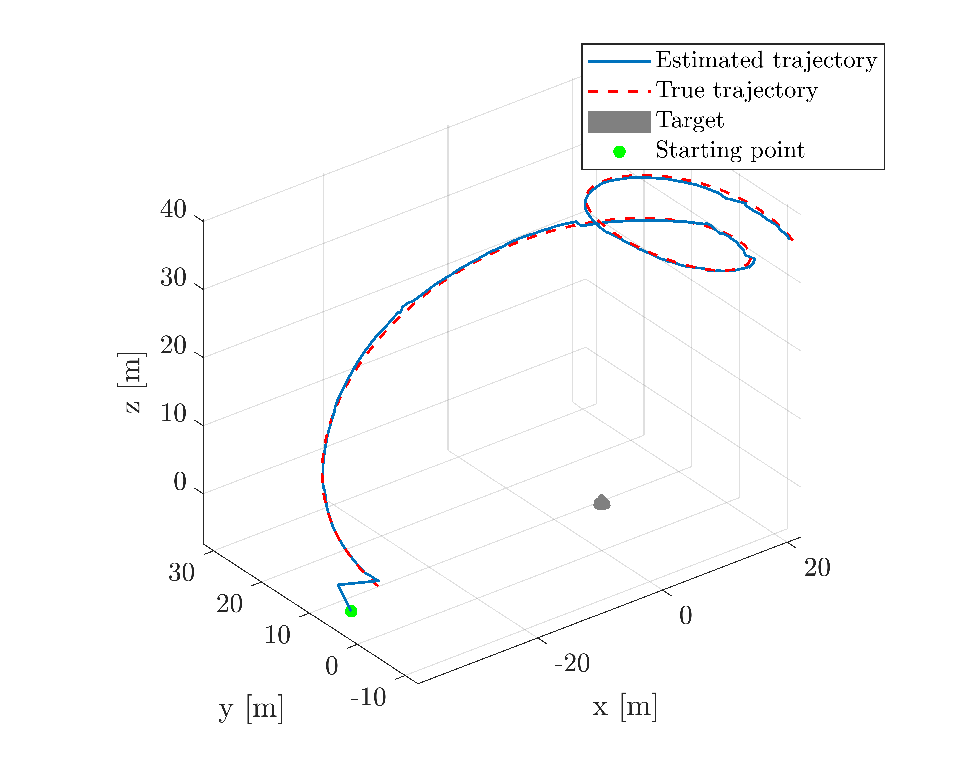
\includegraphics[width = .7\linewidth]{Images/esttraj.eps}
%     \caption{Ground truth and estimate trajectory in the multispectral case}
%     \label{fig:esttraj}
% \end{figure}
% In figure \cref{fig:estimations}, the estimates and the ground truth for each parameter estimated by the filter is reported. 
% The worst results are obtained in terms of estimation of the velocities and angular velocities. This is an expected result as the filter has no direct measurement of these states, and the dynamical models, especially for the angular velocities, are very simplified. The estimated values by the filter are reported in \cref{fig:err_pos}. In the case of the velocity of the center of mass it would be possible to further tune the process noise covariance matrix to rely more on the filter's dynamic, however, because of the elevated initial error and the low convergence, it degrades the position estimation. For the angular rates, to rely more on the angular velocities implies inserting a delay in the angular velocities, as the dynamic of the filter acts as a low pass filter. This delay deteriorates also the results in terms of attitude estimation.\\
% The advantage of having good angular rates estimation is that it give the possibility to estimate the inertia matrix of the target, enabling access to a more precise relative dynamic and safer capture operations. The inertia estimation process is outside of the scope of the thesis but would provide an interesting development of the work.\\
% \begin{figure}[!h]
%     \centering
%     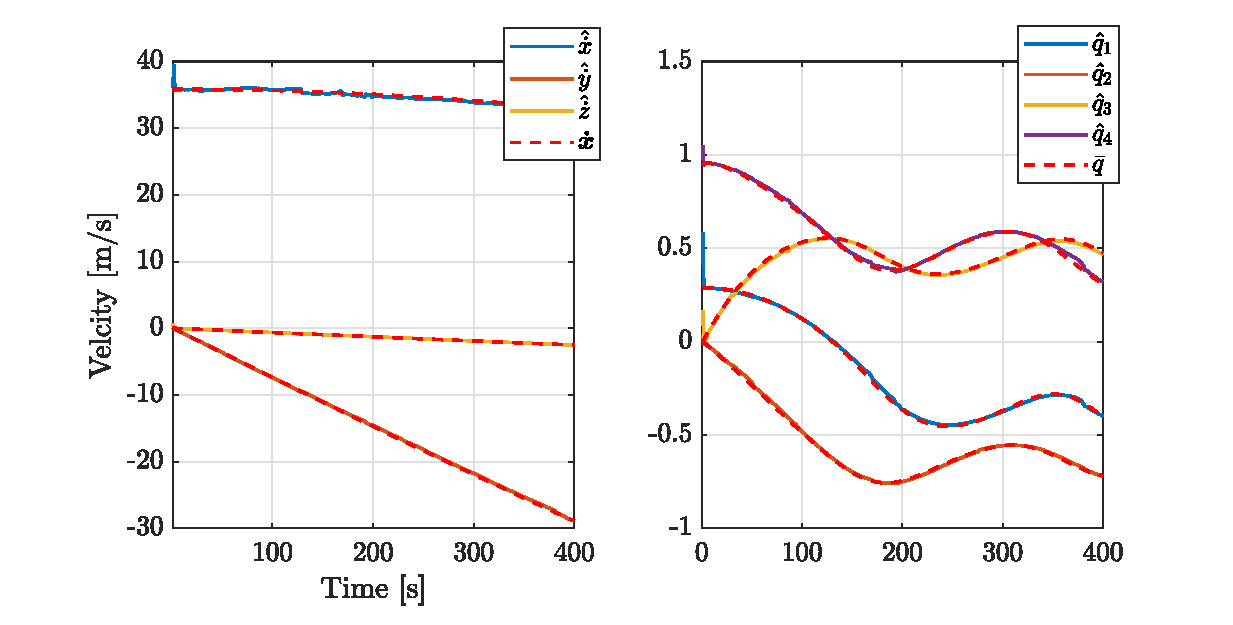
\includegraphics[width=\linewidth]{Images/posatt.eps}
%     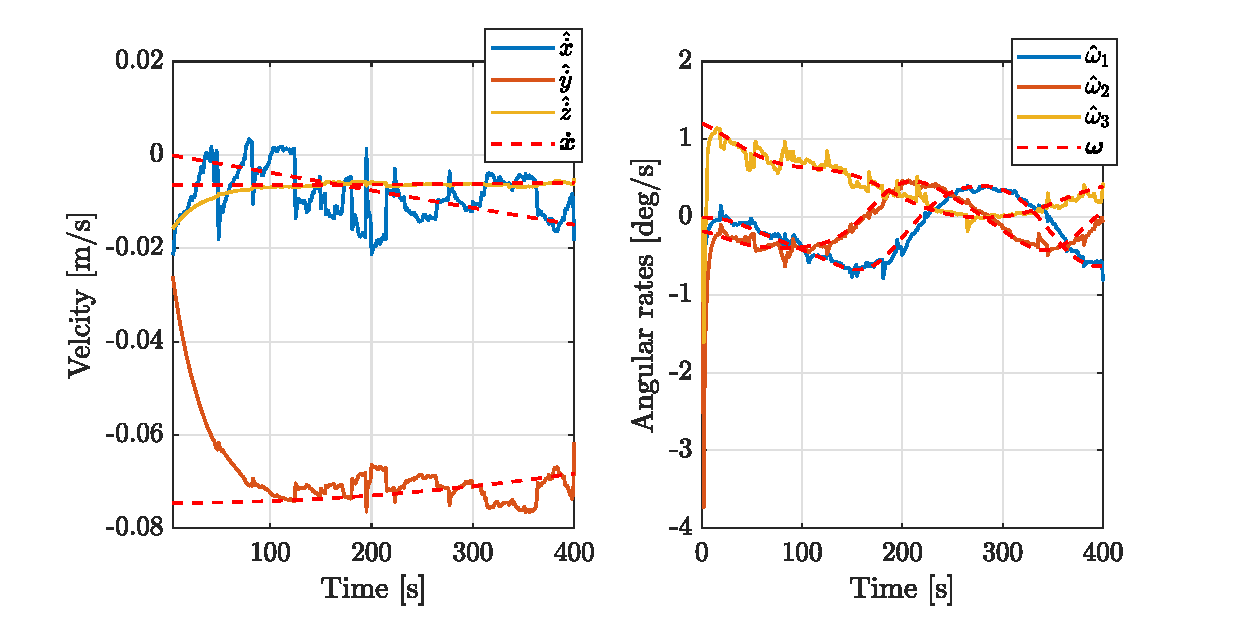
\includegraphics[width=\linewidth]{Images/velrate.eps}
%     \caption{Velocity and angular rates estimated by the filter in the multispectral case }
%     \label{fig:estimations}
% \end{figure}
% In \cref{fig:colors} are graphically reported the variances values associated to the features points processed in association with the visible and thermal measurements. Its possible to observe how the values are of the same order of magnitude as the value given for the initialization. A significant difference can be observed both in terms of variance values and in the overall behaviour of the visible and thermal spectrum. As described in the following section, this is the result of both a lower quality of the thermal images, but also of a significant differences in the working of the IP routine for the two spectra, reducing even more the performances of the TIR sensor. 
% \begin{figure}[!h]
%     \centering
%     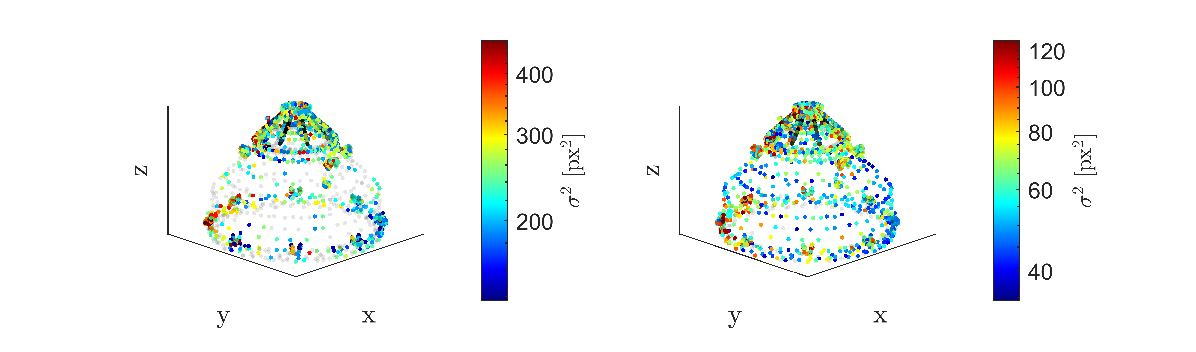
\includegraphics[clip,trim = 2cm 0cm 1cm 0cm,width=\linewidth]{Images/colorful1.eps}
%     \caption{Variance of the features at the end of the simulation for VIS (left) and TIR (right)}
%     \label{fig:colors}
% \end{figure}
% As the algorithm is intended for online pose estimation, it is important that the computational time is lower than the filter update frequency of $\SI{1}{\hertz}$. Although the code is not run on relevan hardware, the CPU time has been computed and reported in \cref{tab:Ctimes} for both the filter steps, including the IP routine, and the multiple re-initialization processes.\\
% As expected the time required for the filter in the case of the multispectral application is higher, as the code executes roughly double to processes with respect to the case of VIS-only or TIR-only. The time required for the re-initialization represents a very critical factors, as it is almost ten times the update step of the filter. Even though this process could be parallelized with respect to the filter execution, while tracking the remaining features, it would be still represent a major issue. 
% \begin{table}[!h]
%     \begin{subtable}[h]{0.42\textwidth}
%         \centering
%         \begin{tabular}{l  c }
%         Spectrum & CPU Time [$\SI{}{\second}$]\\ \hline \hline
%         VIS \& TIR &  $0.17\pm 0.03$\\\hline
%         VIS &  $0.08\pm 0.02$ \\\hline
%         TIR &  $0.07\pm 0.02$ \\\hline
%         \end{tabular}
%         \caption{Filter's step computational time}
%         \label{tab:Csteps}
%      \end{subtable}
%     \hfill
%     \begin{subtable}[h]{0.42\textwidth}
%         \centering
%         \begin{tabular}{l  c }
%         Spectrum & CPU Time [$\SI{}{\second}$]\\ \hline \hline
%         VIS &  $8.9\pm 0.55$ \\\hline
%         TIR &  $9.0\pm 0.46$ \\\hline
%         \end{tabular}
%         \caption{re-initialization computational time}
%         \label{tab:Creinit}
%      \end{subtable}
%      \caption{Position and attitude errors for the different spectrum modalities}
%      \label{tab:Ctimes}
% \end{table}
% \begin{figure}[!h]
%     \centering
%     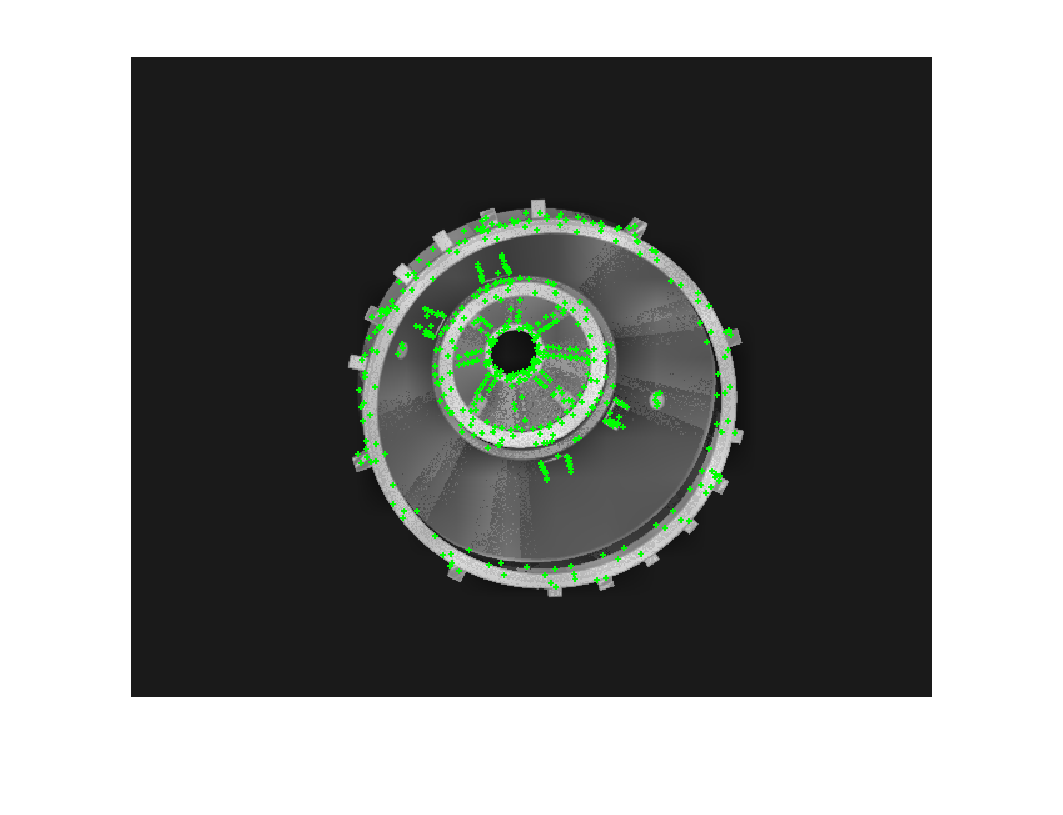
\includegraphics[width=\linewidth]{Images/TIRDownVespa.eps}
%     \includegraphics[width=.6\linewidth]{Images/TRIupVespa.eps}
%     \caption{Velocity and angular rates estimated by the filter in the multispectral case }
%     \label{fig:estimations}
% \end{figure}
